% !TeX encoding = UTF-8
% !TeX program = pdflatex
% Maestro final del TFM. Antes del depósito, incorporar aquí la portada oficial,
% el nombre del máster, la institución y la dirección académica.
\documentclass[12pt,a4paper,twoside,openany]{book}

% -----------------------------------------------------------------------------
% Codificación, idioma y tipografía
% -----------------------------------------------------------------------------
\usepackage[utf8]{inputenc}
\usepackage[T1]{fontenc}
\usepackage[spanish,es-nodecimaldot]{babel}
\usepackage{lmodern}
\usepackage{microtype}
\usepackage{csquotes}
\usepackage{xspace}

% -----------------------------------------------------------------------------
% Página y composición
% -----------------------------------------------------------------------------
\usepackage[a4paper,inner=2.5cm,outer=2.5cm,top=3cm,bottom=3cm,
            headheight=28pt]{geometry}
\usepackage{setspace}
\onehalfspacing
\setlength{\parindent}{0.65cm}
\setlength{\parskip}{0pt}
\widowpenalty=10000
\clubpenalty=10000
\displaywidowpenalty=10000
\emergencystretch=2em
\raggedbottom
\usepackage{fancyhdr}
\usepackage{emptypage}
\pagestyle{fancy}
\fancyhf{}
\fancyhead[LE]{\small\thepage\quad\textsc{Resolución numérica de llamas}}
\fancyhead[RO]{\small\textsc{\leftmark}\quad\thepage}
\renewcommand{\headrulewidth}{0.4pt}
\fancypagestyle{plain}{%
  \fancyhf{}
  \fancyfoot[C]{\thepage}
  \renewcommand{\headrulewidth}{0pt}}

% -----------------------------------------------------------------------------
% Matemática, unidades, tablas y gráficos
% -----------------------------------------------------------------------------
\usepackage{amsmath,amssymb,mathtools,bm}
\usepackage{siunitx}
\sisetup{output-decimal-marker={,},per-mode=symbol,detect-all=true}
\DeclareSIUnit\atmosphere{atm}
\usepackage{booktabs,array,longtable,tabularx,multirow}
\newcolumntype{Y}{>{\raggedright\arraybackslash}X}
\newcolumntype{C}{>{\centering\arraybackslash}X}
\usepackage{graphicx}
\graphicspath{{figuras/}{revision_figures/}}
\usepackage{float}
\usepackage{pdflscape}
\usepackage[section]{placeins}
\usepackage[font=small,labelfont=bf]{caption}
\usepackage{subcaption}
\usepackage{xcolor}
\definecolor{azulTFM}{HTML}{155C8A}
\definecolor{azulElectrico}{HTML}{0066FF}
\definecolor{verdeTFM}{HTML}{2D7F5E}
\definecolor{naranjaTFM}{HTML}{D97706}
\usepackage{tikz}
\usetikzlibrary{arrows.meta,positioning,shapes.geometric,fit,calc,babel,decorations.pathreplacing}

% Estilos comunes de los diagramas numéricos detallados.
\tikzset{
  num block/.style={rectangle,rounded corners=3pt,draw=azulTFM,
    fill=azulTFM!5,line width=.8pt,align=center,text width=4.2cm,
    minimum height=.9cm,inner sep=5pt},
  num decision/.style={diamond,aspect=2.6,draw=naranjaTFM,
    fill=naranjaTFM!8,line width=.8pt,align=center,text width=2.7cm,inner sep=1.5pt},
  num end/.style={num block,draw=verdeTFM,fill=verdeTFM!8},
  num fail/.style={num block,draw=red!65!black,fill=red!4},
  num arrow/.style={-{Latex[length=2.2mm]},draw=black!70,line width=.8pt},
  num tag/.style={font=\scriptsize,fill=white,inner sep=1.5pt}
}

\usepackage{pgfplots}
\pgfplotsset{compat=1.18}
\usepackage{pgfplotstable}

% -----------------------------------------------------------------------------
% Listas y enlaces
% -----------------------------------------------------------------------------
\usepackage{enumitem}
\setlist{itemsep=0.25em,topsep=0.35em}
\usepackage[unicode]{hyperref}
\hypersetup{
  colorlinks=true,
  linkcolor=blue,
  citecolor=blue,
  urlcolor=blue,
  filecolor=blue,
  pdftitle={Resolución numérica de llamas premezcladas en régimen laminar},
  pdfauthor={Kevin Vidal},
  pdfsubject={Llamas premezcladas laminares, métodos numéricos, solver unidimensional y FGM},
  pdfkeywords={FGM, flamelet, Cantera, PTC-SER, Newton, HPC, combustión}
}
\usepackage[spanish,nameinlink,noabbrev,capitalise]{cleveref}
\crefname{chapter}{Chapter}{Chapters}
\Crefname{chapter}{Chapter}{Chapters}
\crefname{section}{Section}{Sections}
\Crefname{section}{Section}{Sections}
\crefname{figure}{Fig.}{Figs.}
\Crefname{figure}{Fig.}{Figs.}
\crefname{table}{Table}{Tables}
\Crefname{table}{Table}{Tables}
\crefname{equation}{Eq.}{Eqs.}
\Crefname{equation}{Eq.}{Eqs.}

% -----------------------------------------------------------------------------
% Macros y convenciones
% -----------------------------------------------------------------------------
\newcommand{\vect}[1]{\bm{#1}}
\newcommand{\mat}[1]{\bm{#1}}
\newcommand{\dd}{\mathop{}\!\mathrm{d}}
\newcommand{\pd}[2]{\frac{\partial #1}{\partial #2}}
\newcommand{\norm}[1]{\left\lVert #1\right\rVert}
\newcommand{\abs}[1]{\left\lvert #1\right\rvert}
\newcommand{\Su}{S_{\mathrm{u}}}
\newcommand{\Tin}{T_{\mathrm{in}}}
\newcommand{\Tad}{T_{\mathrm{ad}}}
\newcommand{\Yk}{Y_k}
\newcommand{\omegak}{\dot{\omega}_k}
\newcommand{\FGM}{\textsc{FGM}\xspace}
\newcommand{\KFLAME}{\textsc{KFLAME}\xspace}
\newcommand{\Cantera}{\textsc{Cantera}\xspace}
\newcommand{\codigo}[1]{\texttt{#1}}

\DeclareRobustCommand{\numref}[3]{\hyperlink{flow:#1:#2}{Fig.~\ref*{#1}: #3}}

% Páginas A4 realmente horizontales: los destinos PDF no dependen de una
% rotación de la caja de texto (que desplaza los enlaces de hyperref).
\newcommand{\BeginNumLandscape}{%
  \clearpage
  \newgeometry{layoutwidth=297mm,layoutheight=210mm,
    left=25mm,right=25mm,top=25mm,bottom=25mm,headheight=28pt}%
  \pdfpagewidth=297mm\pdfpageheight=210mm
  \paperwidth=297mm\paperheight=210mm
  \setlength{\headwidth}{\textwidth}%
}
\newcommand{\EndNumLandscape}{%
  \clearpage
  \pdfpagewidth=210mm\pdfpageheight=297mm
  \paperwidth=210mm\paperheight=297mm
  \restoregeometry
  \setlength{\headwidth}{\textwidth}%
}

% Las tablas generadas no están presentes en esta copia. Esta orden las carga
% cuando existen y permite compilar el documento cuando no fueron copiadas.
\providecommand{\SweepReportRoot}{../../../runs/thesis_flames_L3/report_expanded}
\newcommand{\InputGeneratedTable}[1]{%
  \IfFileExists{\SweepReportRoot/#1}{%
    \input{\SweepReportRoot/#1}%
  }{%
    \PackageWarningNoLine{TFM}{No se encontro la tabla generada #1}%
  }%
}

\begin{document}
\hypersetup{pageanchor=false}

\chapter{Resultados}
\label{chap:resultados}
\chaptermark{Resultados}

Los resultados se organizan de forma progresiva, comenzando con la verificación
numérica de las llamas individuales y continuando con la evaluación de su coste
computacional; sobre esta base se aborda posteriormente la construcción y
evaluación del modelo FGM.

% =============================================================================
\section{Llamas individuales}
\label{sec:individual-flames-results}
% =============================================================================

% -----------------------------------------------------------------------------
\subsection{Verificación numérica}
\label{sec:numerical-verification}
% -----------------------------------------------------------------------------

La verificación comienza con el estudio de sensibilidad espacial, a partir del
cual se selecciona el nivel de refinamiento utilizado en las evaluaciones
posteriores; una vez fijada esta discretización, la comparación con
\Cantera{} se examina primero sobre casos representativos y después se extiende
al conjunto completo de condiciones mediante las métricas definidas en la
\cref{sec:individual-flame-verification}.

\paragraph{Sensibilidad de malla y dominio}

La sensibilidad espacial se evalúa con \(\phi=1\) en seis estados, tres por
mecanismo: \SI{1}{\atmosphere} y \SI{300}{\kelvin},
\SI{10}{\atmosphere} y \SI{300}{\kelvin}, y
\SI{1}{\atmosphere} y \SI{500}{\kelvin}; para CH$_4$--aire con
GRI-Mech~3.0 se emplea transporte promediado sin Soret, mientras que para
H$_2$--aire con \texttt{h2o2.yaml} se utiliza transporte multicomponente con
Soret. En cada estado se comparan los niveles L2--L5 definidos en la
\cref{tab:mesh-refinement-levels} y, de forma independiente, se repite L3
duplicando la longitud inicial del dominio, tomando la solución L3 de cada
solver como referencia. La \cref{fig:rev-11-sensibilidad-L3} permite observar
cualitativamente cómo cambian \(\Su\) y \(T_b\) al aumentar el refinamiento y
al duplicar la extensión inicial del dominio, mientras que la
\cref{tab:spatial-sensitivity-summary} cuantifica estas variaciones mediante
las diferencias entre L5 y L3, el número de nodos, \(E_2(T)\) y el cambio de
\(\Su\) asociado a la repetición de L3 con \(2L\).

\begin{figure}[!htbp]
\centering
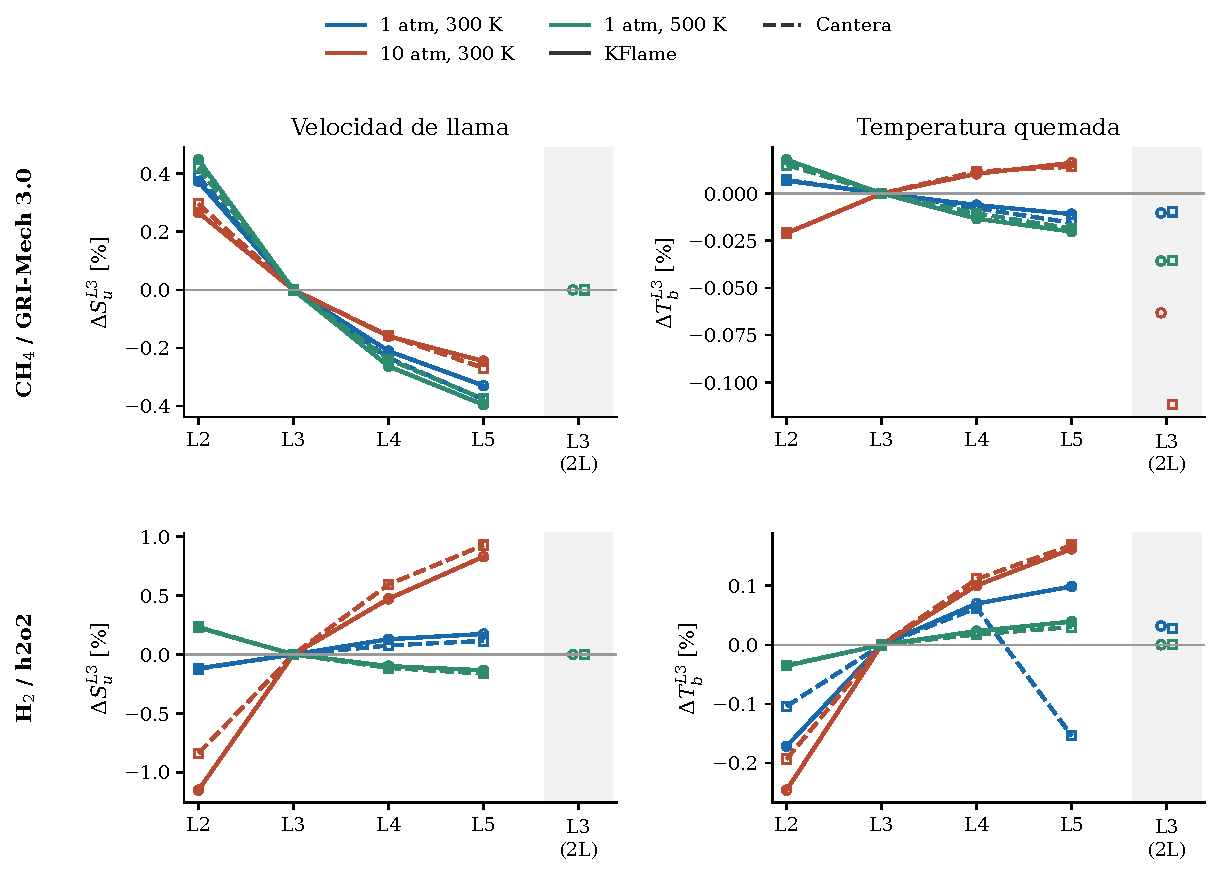
\includegraphics[
    width=\textwidth,
    height=.70\textheight,
    keepaspectratio
]{revision_figures/11_sensibilidad_L3.pdf}
\caption{Sensibilidad espacial respecto a L3 para CH$_4$--aire con transporte
promediado sin Soret y H$_2$--aire con transporte multicomponente y Soret, al
modificar el nivel de refinamiento y duplicar la longitud inicial del dominio.}
\label{fig:rev-11-sensibilidad-L3}
\end{figure}

\begin{table}[!htbp]
\centering
\scriptsize
\caption{Sensibilidad espacial respecto a L3. Las columnas K/C corresponden a
\KFLAME{}/\Cantera{}, respectivamente.}
\label{tab:spatial-sensitivity-summary}
\resizebox{\textwidth}{!}{%
\begin{tabular}{@{}lccccc@{}}
\toprule
Estado &
\(N_{\mathrm{L3}}\) K/C &
\(\left|\Delta S_u^{\mathrm{L5-L3}}\right|\) [\si{\percent}] K/C &
\(\Delta T_b^{\mathrm{L5-L3}}\) [\si{\percent}] K/C &
\(E_2(T)\) [\si{\percent}] K/C &
\(\left|\Delta S_u^{2L-\mathrm{L3}}\right|\) [\si{\percent}] K/C \\
\midrule

CH$_4$, 1 atm, 300 K
& 966 / 987
& 0.330 / 0.377
& $-0.0109$ / $-0.0156$
& 0.011 / 0.012
& \num{5.8e-5} / \num{9.3e-6} \\

CH$_4$, 10 atm, 300 K
& 1047 / 968
& 0.245 / 0.269
& $+0.0162$ / $+0.0141$
& 0.018 / 0.016
& \num{2.5e-10} / \num{4.6e-8} \\

CH$_4$, 1 atm, 500 K
& 973 / 939
& 0.395 / 0.376
& $-0.0202$ / $-0.0186$
& 0.015 / 0.014
& \num{2.8e-4} / \num{9.6e-6} \\

H$_2$, 1 atm, 300 K
& 705 / 722
& 0.174 / 0.115
& $+0.0987$ / $-0.1535$
& 0.104 / 0.087
& \num{3.6e-9} / \num{3.2e-6} \\

H$_2$, 10 atm, 300 K
& 723 / 730
& 0.830 / 0.928
& $+0.1621$ / $+0.1685$
& 0.161 / 0.167
& \num{9.3e-12} / \num{5.5e-7} \\

H$_2$, 1 atm, 500 K
& 690 / 710
& 0.134 / 0.163
& $+0.0394$ / $+0.0301$
& 0.056 / 0.045
& \num{5.2e-12} / \num{3.1e-10} \\

\bottomrule
\end{tabular}%
}
\end{table}

Al duplicar la longitud inicial del dominio, la variación máxima de \(\Su\) es
de \SI{2.8e-4}{\percent}, lo que confirma una influencia despreciable de su
extensión inicial sobre esta magnitud; entre L3 y L5, los tres estados de
CH$_4$ y los casos de H$_2$ a \SI{1}{\atmosphere} mantienen cambios de
\(\Su\) inferiores a \SI{0.40}{\percent}, mientras que para H$_2$ a
\SI{10}{\atmosphere} se alcanzan \SI{0.83}{\percent} en \KFLAME{} y
\SI{0.93}{\percent} en \Cantera{}. Las variaciones térmicas permanecen por
debajo de \SI{0.17}{\percent} para \(\left|\Delta T_b\right|\) y de
\SI{0.167}{\percent} para \(E_2(T)\), resultados que se contrastan con el
coste computacional de cada nivel en la \cref{fig:rev-mesh-time}.

\begin{figure}[!htbp]
\centering
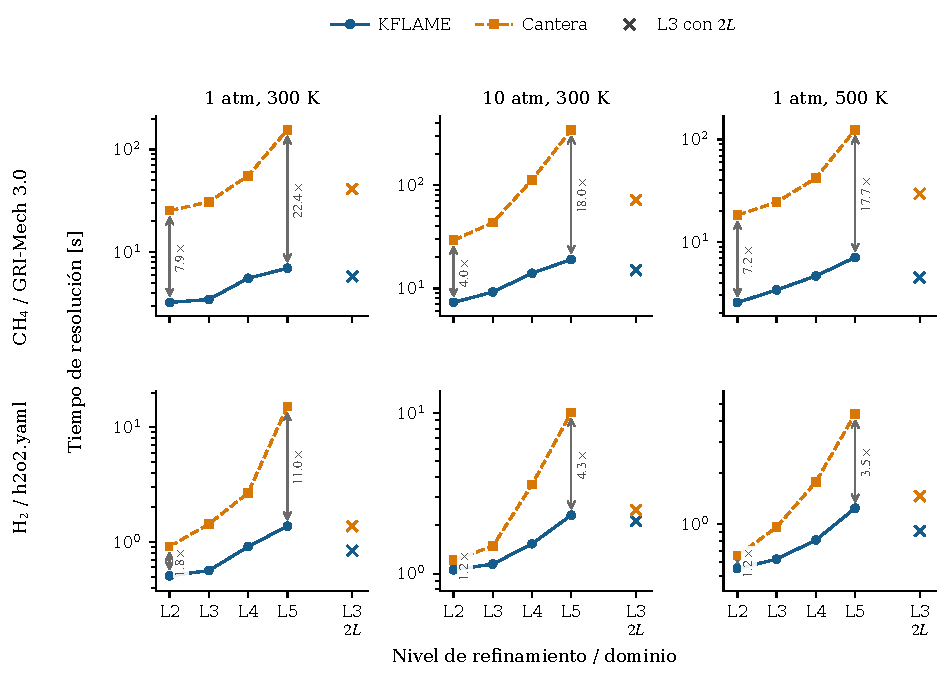
\includegraphics[
    width=\textwidth,
    height=.95\textheight,
    keepaspectratio
]{revision_figures/tiempo_vs_malla.pdf}
\caption{Tiempo de resolución frente al nivel de refinamiento para los seis
estados del estudio de sensibilidad. La fila superior corresponde a
CH$_4$--aire con transporte promediado sin Soret y la inferior a
H$_2$--aire con transporte multicomponente y Soret; las cruces representan
las repeticiones de L3 con la longitud inicial del dominio duplicada.}
\label{fig:rev-mesh-time}
\end{figure}

Entre L3 y L5, el tiempo de \KFLAME{} aumenta aproximadamente entre
\(2.0\) y \(2.4\) veces, mientras que en \Cantera{} lo hace entre
\(4.6\) y \(10.6\) veces; este incremento contrasta con las variaciones de
\(\Su\), \(T_b\) y \(E_2(T)\) observadas entre ambos niveles, por lo que L3 se
adopta para las evaluaciones posteriores como compromiso entre resolución
espacial y tiempo de cálculo, manteniendo identificada la mayor sensibilidad
del H$_2$ a \SI{10}{\atmosphere}.

\FloatBarrier

\paragraph{Comparación con \Cantera{} en casos representativos}

Con el nivel L3 seleccionado, la concordancia entre ambas implementaciones se
evalúa inicialmente para llamas de CH$_4$--aire y H$_2$--aire a
\(\phi=1\), \SI{1}{\atmosphere} y \SI{300}{\kelvin}, considerando en cada
mecanismo las cuatro configuraciones de transporte. Los perfiles se alinean
respecto al punto medio térmico mediante la \cref{eq:profile-alignment} y su
concordancia se cuantifica con \(\delta_{S_u}\), \(E_2(T)\),
\(E_2(\dot q)\) y \(\max_k E_2(Y_k)\), de acuerdo con la
\cref{eq:profile-concordance}; las
\cref{fig:rev-02-perfiles-CH4,fig:rev-02-perfiles-H2} reúnen para ambos
mecanismos la temperatura, la velocidad local, las principales especies y la
liberación de calor, junto con las métricas correspondientes.

\begin{figure}[!htbp]
\centering
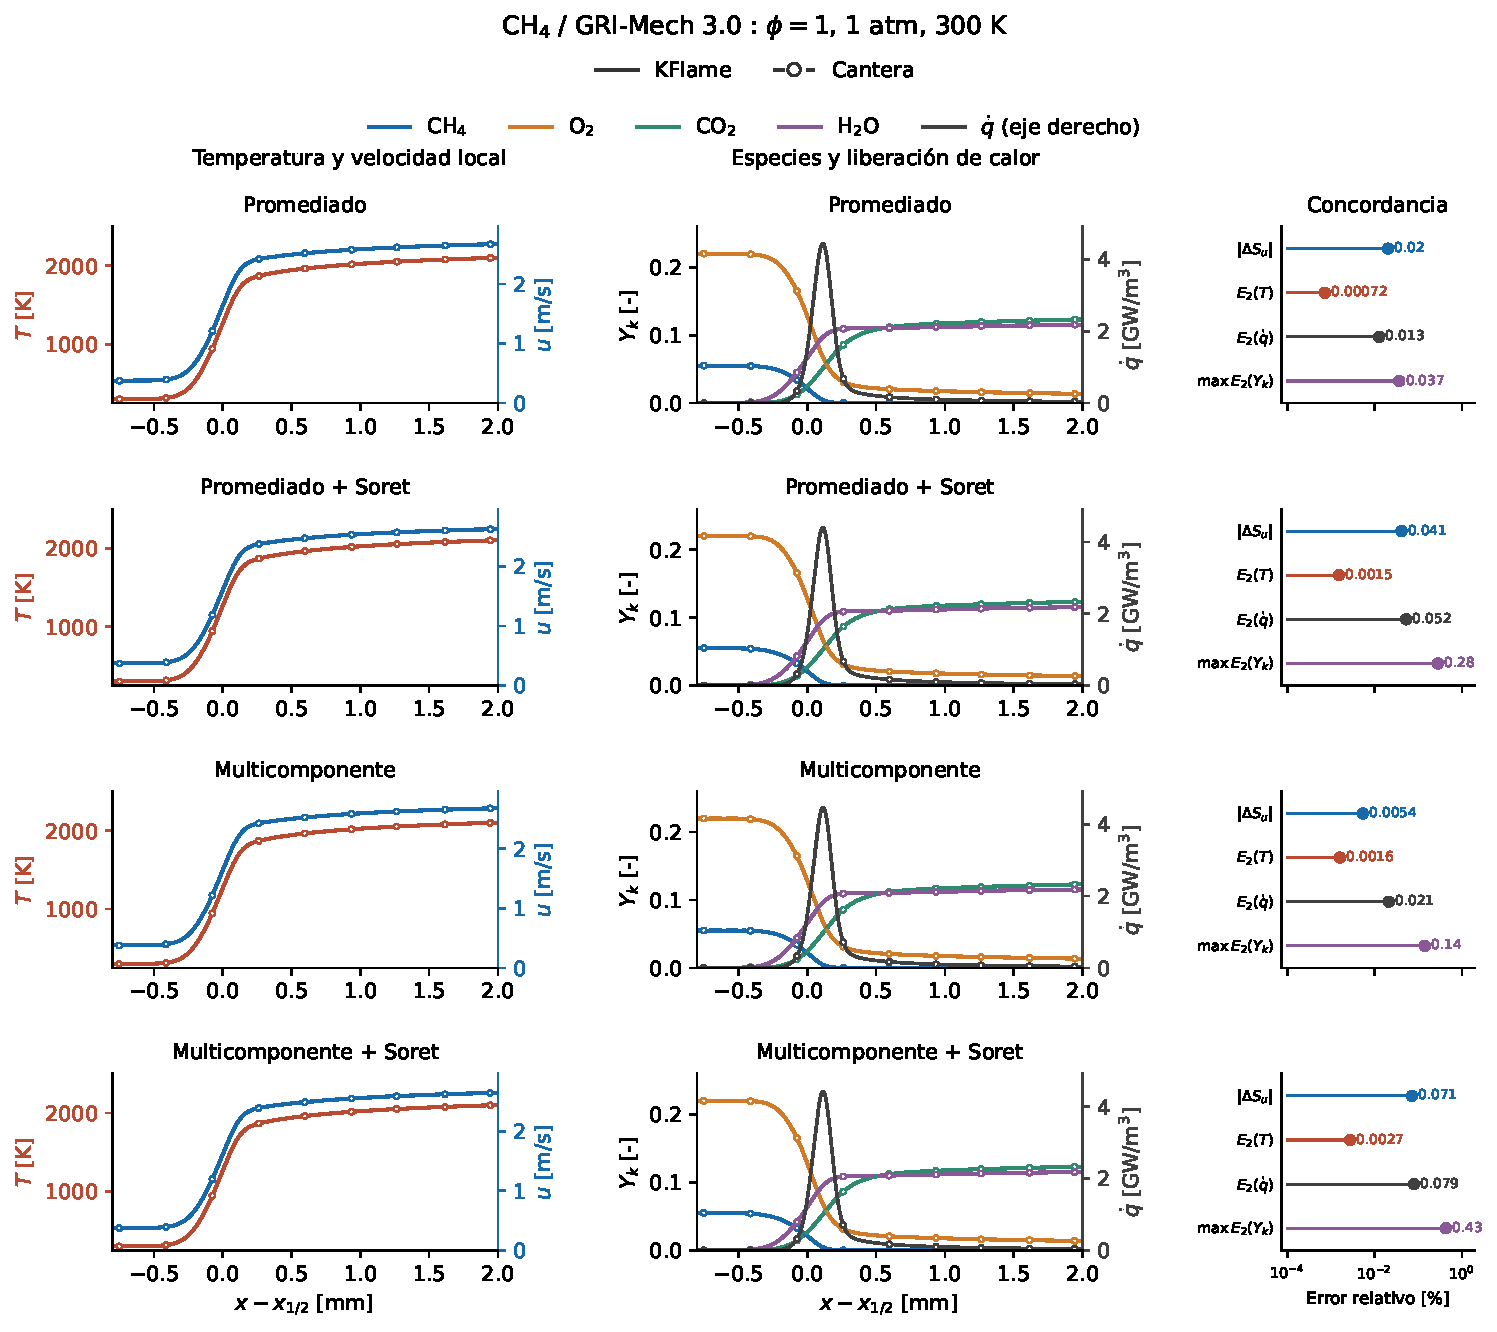
\includegraphics[
    width=\textwidth,
    height=.90\textheight,
    keepaspectratio
]{revision_figures/02_perfiles_CH4.pdf}
\caption{Comparación entre \KFLAME{} y \Cantera{} para CH$_4$--aire en las
cuatro configuraciones de transporte. Las dos primeras columnas muestran los
perfiles alineados respecto a \(x_{1/2}\), mientras que la tercera presenta
\(\delta_{S_u}\), \(E_2(T)\), \(E_2(\dot q)\) y
\(\max_k E_2(Y_k)\).}
\label{fig:rev-02-perfiles-CH4}
\end{figure}

\begin{figure}[!htbp]
\centering
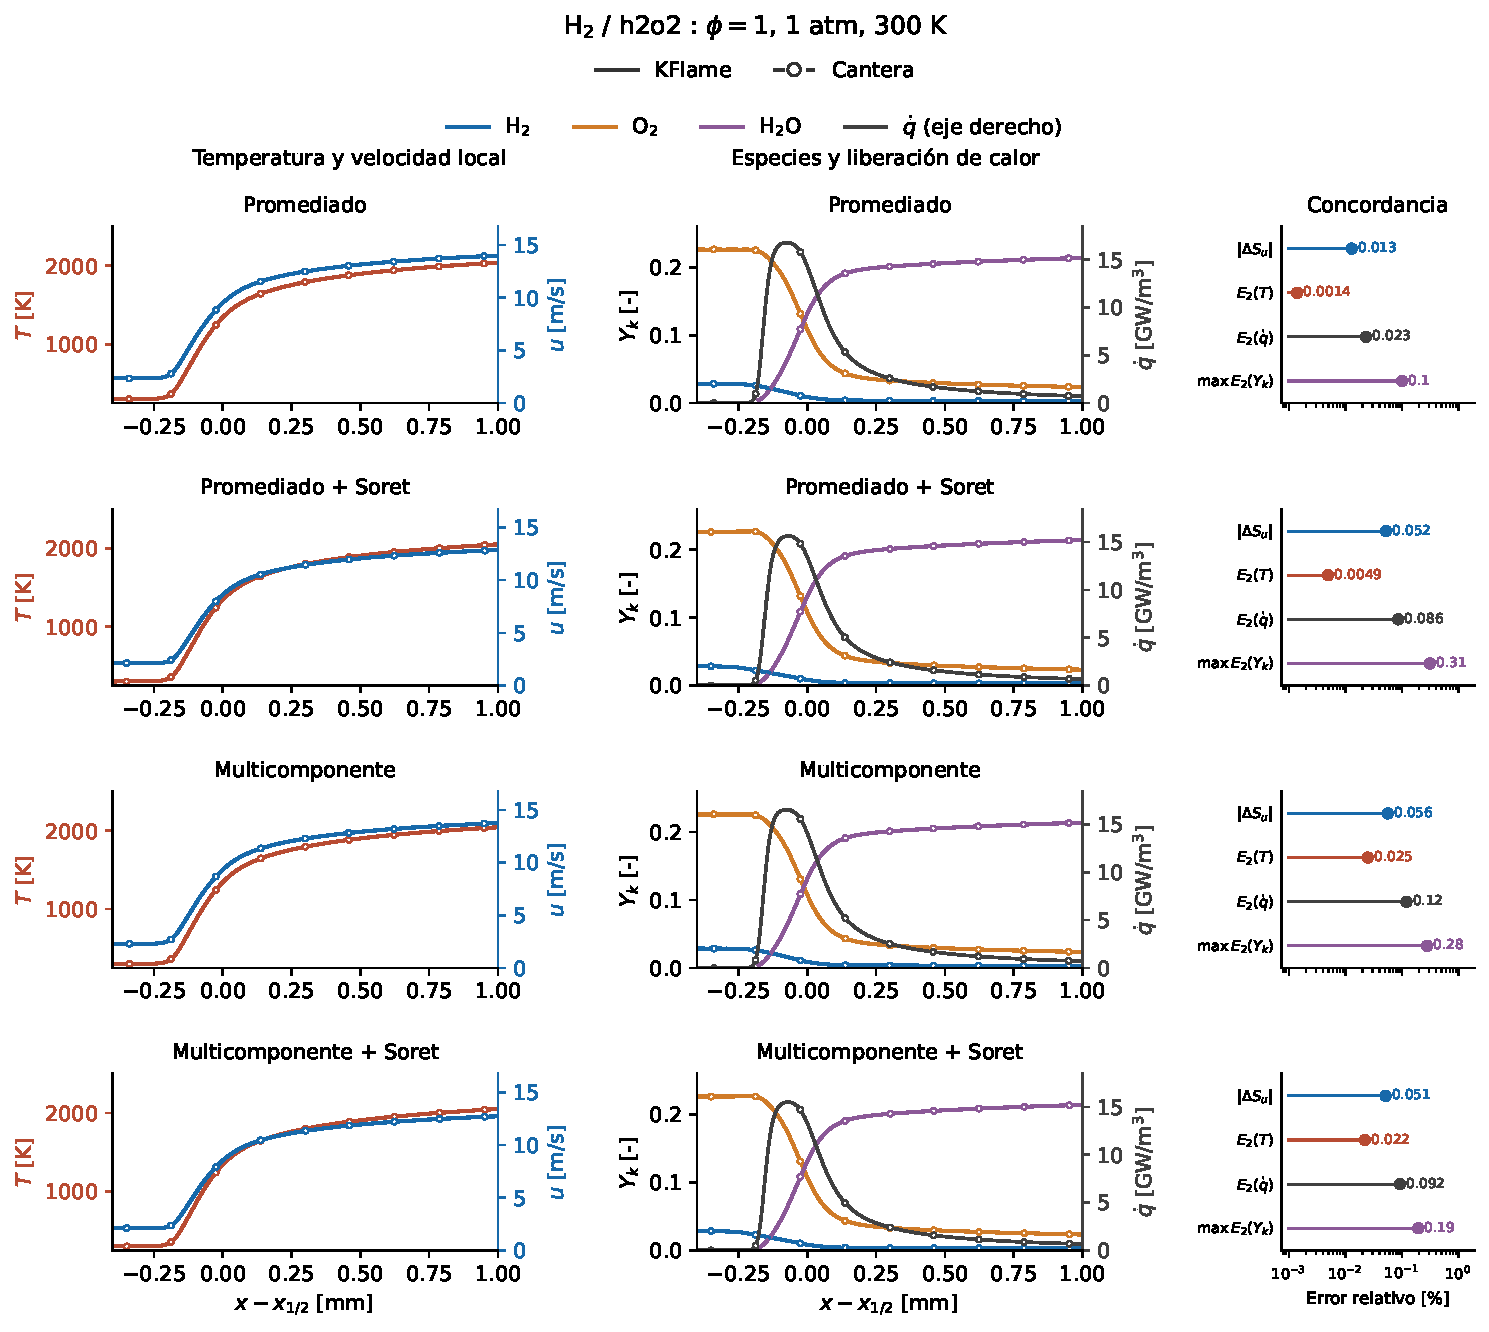
\includegraphics[
    width=\textwidth,
    height=.90\textheight,
    keepaspectratio
]{revision_figures/02_perfiles_H2.pdf}
\caption{Comparación entre \KFLAME{} y \Cantera{} para H$_2$--aire en las
cuatro configuraciones de transporte. Las dos primeras columnas muestran los
perfiles alineados respecto a \(x_{1/2}\), mientras que la tercera presenta
\(\delta_{S_u}\), \(E_2(T)\), \(E_2(\dot q)\) y
\(\max_k E_2(Y_k)\).}
\label{fig:rev-02-perfiles-H2}
\end{figure}

En ambos mecanismos, \KFLAME{} y \Cantera{} reproducen una evolución próxima
de las variables a través del frente para las cuatro configuraciones de
transporte, con las mayores discrepancias relativas concentradas en las
especies y diferencias menores en la temperatura y la velocidad de llama;
esta comparación no requiere que ambas implementaciones generen la misma
discretización espacial, como muestra la
\cref{fig:rev-10-mallas-finales}, donde se presenta su distribución alrededor
del frente para dos configuraciones representativas.

\begin{figure}[!htbp]
\centering
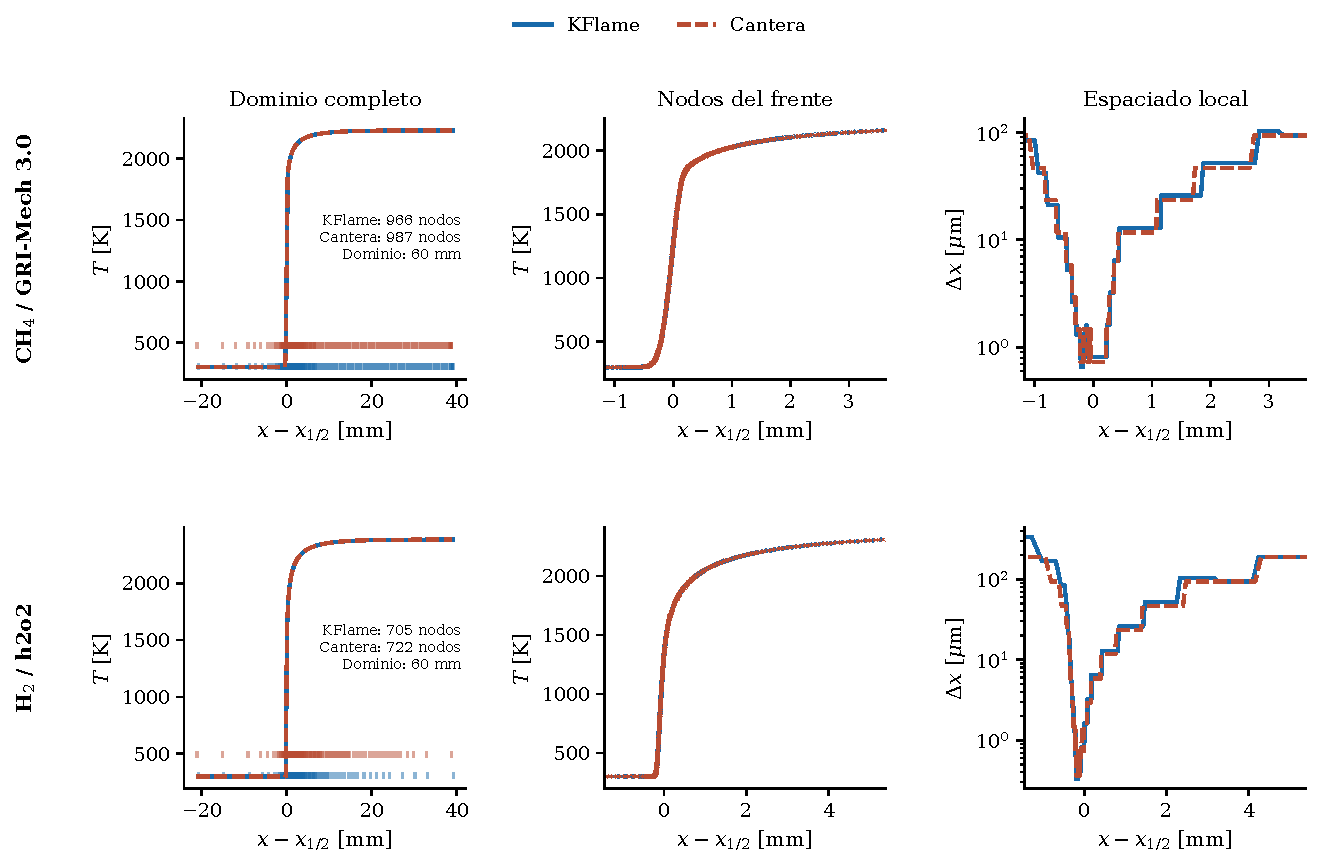
\includegraphics[
    width=\textwidth,
    height=.90\textheight,
    keepaspectratio
]{revision_figures/10_mallas_finales.pdf}
\caption{Distribución espacial de la discretización para CH$_4$--aire con
transporte promediado sin Soret y H$_2$--aire con transporte multicomponente y
Soret, expresada respecto al punto medio térmico \(x_{1/2}\).}
\label{fig:rev-10-mallas-finales}
\end{figure}

Ambas implementaciones concentran la discretización alrededor del frente,
aunque las posiciones nodales resultantes no coinciden exactamente, lo que
justifica la alineación e interpolación sobre una coordenada espacial común
antes de evaluar la concordancia de los perfiles. Para estos mismos ocho casos
representativos, las ejecuciones instrumentadas permiten además cuantificar el
trabajo realizado por cada solver y relacionarlo con la distribución del tiempo
de resolución; la \cref{fig:rev-17-trabajo-por-llama} reúne las evaluaciones
del residual, las construcciones del Jacobiano, el tiempo medio por
construcción y los pasos Euler aceptados.

\begin{figure}[p]
\centering
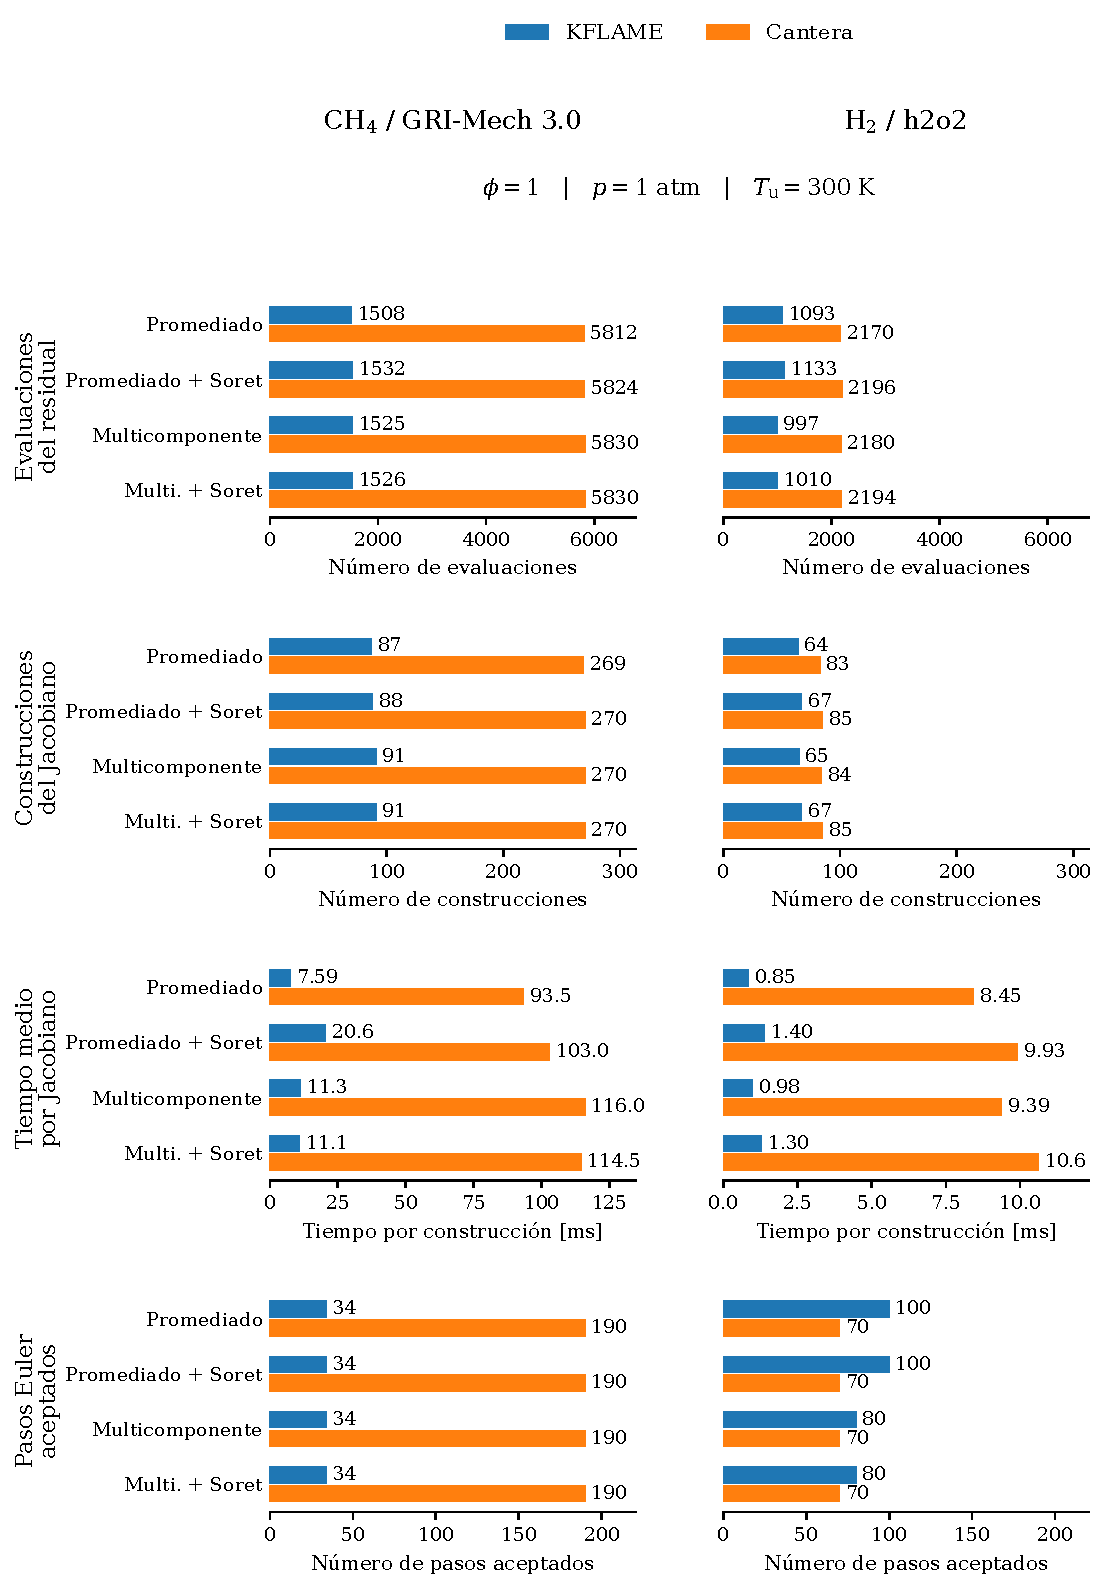
\includegraphics[
    width=\textwidth,
    height=.84\textheight,
    keepaspectratio
]{revision_figures/17_trabajo_por_llama_a4.pdf}
\caption{Trabajo computacional registrado en las mismas ejecuciones
instrumentadas de los ocho casos representativos para \KFLAME{} y
\Cantera{}. Se muestran las evaluaciones del residual, las construcciones del
Jacobiano, el tiempo medio por construcción y los pasos Euler aceptados para
las cuatro configuraciones de transporte.}
\label{fig:rev-17-trabajo-por-llama}
\end{figure}

La \cref{fig:rev-17-trabajo-por-llama} muestra que la reducción del trabajo
interno es más pronunciada para CH$_4$: frente a \Cantera{}, \KFLAME{}
realiza aproximadamente un \SIrange{73.7}{74.1}{\percent} menos de
evaluaciones del residual y un \SIrange{66.3}{67.7}{\percent} menos de
construcciones del Jacobiano, a lo que se añade una reducción de entre
\SI{80}{\percent} y \SI{92}{\percent} en el tiempo medio necesario para cada
construcción. En H$_2$ la diferencia en el número de operaciones es menor,
con reducciones de aproximadamente \SIrange{48}{54}{\percent} en las
evaluaciones del residual y de \SIrange{21}{23}{\percent} en las
construcciones del Jacobiano, aunque el coste medio de esta última operación
continúa siendo entre un \SI{86}{\percent} y un \SI{90}{\percent} inferior en
\KFLAME{}. Los pasos Euler aceptados muestran además estrategias de
recuperación diferentes entre ambas implementaciones, por lo que su recuento
se utiliza como indicador de la trayectoria de convergencia y no como medida
directa de eficiencia.

Estas diferencias se reflejan en el desglose temporal de las mismas
ejecuciones instrumentadas, presentado en la
\cref{fig:rev-16-origen-coste}.

\begin{figure}[!htbp]
\centering
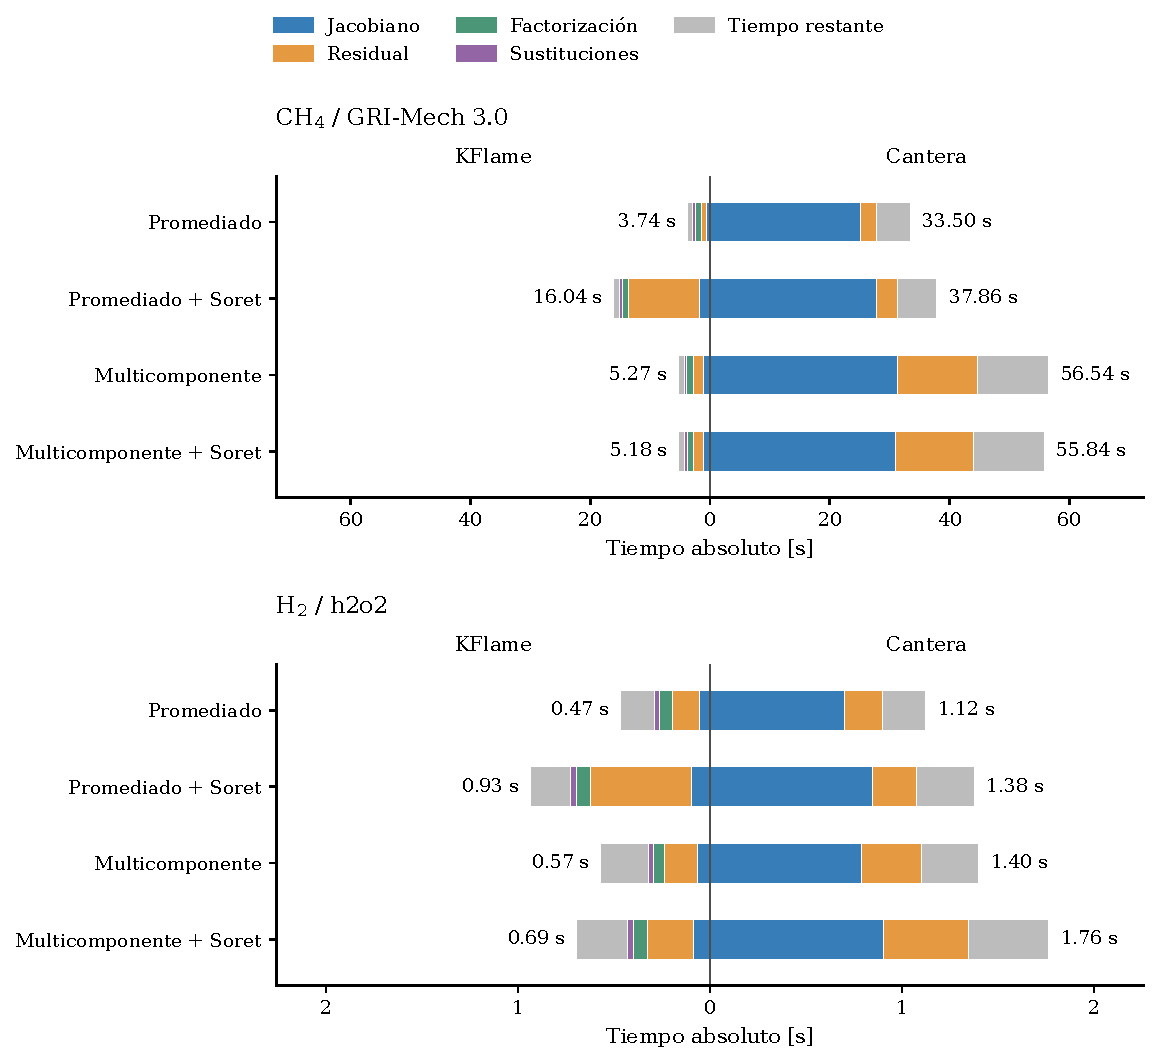
\includegraphics[
    width=\textwidth,
    height=.70\textheight,
    keepaspectratio
]{revision_figures/16_origen_coste.pdf}
\caption{Distribución del tiempo de las mismas ejecuciones instrumentadas de
los ocho casos representativos. En \KFLAME{} se separan el residual, la
construcción del Jacobiano, la factorización y las sustituciones, mientras que
en \Cantera{} las operaciones sin temporización independiente, incluidas las
asociadas al álgebra lineal, permanecen incorporadas en el tiempo restante.}
\label{fig:rev-16-origen-coste}
\end{figure}

El menor trabajo registrado y, especialmente, el menor coste de construcción
del Jacobiano se traducen en reducciones del tiempo total de entre
\SI{58}{\percent} y \SI{91}{\percent} para CH$_4$ y de entre
\SI{33}{\percent} y \SI{61}{\percent} para H$_2$ respecto a \Cantera{}. La
excepción interna más relevante aparece al activar Soret con transporte
promediado en CH$_4$, donde el tiempo total de \KFLAME{} aumenta
aproximadamente un \SI{329}{\percent} respecto al mismo transporte sin Soret,
a pesar de que el número de construcciones del Jacobiano permanece
prácticamente constante; este incremento procede principalmente del residual,
cuyo tiempo pasa de \SI{0.73}{\second} a \SI{11.76}{\second}, es decir, se
multiplica por aproximadamente \(16\), debido a que la evaluación del
transporte y de los flujos en las caras concentra cerca del
\SI{96}{\percent} de su coste. En cambio, con transporte multicomponente la
activación de Soret apenas modifica el tiempo total de \KFLAME{}, lo que
indica que el aumento de coste no está asociado a Soret de forma general, sino
a su interacción con la formulación de transporte promediado.

\FloatBarrier

\paragraph{Campaña numérica}

Verificada la concordancia y caracterizado el comportamiento de los casos
representativos, el análisis se extiende a CH$_4$--aire con GRI-Mech~3.0 y
H$_2$--aire con \texttt{h2o2.yaml} mediante barridos de composición, presión y
temperatura, considerando transporte promediado y multicomponente con Soret
activado y desactivado; la \cref{tab:campaign-design-L3} resume las condiciones
evaluadas y el número de estados únicos aportado por cada barrido.

\begin{table}[!htbp]
\centering
\small
\caption{Configuración de la campaña L3 para ambos mecanismos. Las condiciones
únicas consideran las cuatro configuraciones de transporte y excluyen los
estados coincidentes entre barridos.}
\label{tab:campaign-design-L3}
\resizebox{\textwidth}{!}{%
\begin{tabular}{@{}lccc cc@{}}
\toprule
Barrido &
Valores &
Condiciones fijas &
\multicolumn{2}{c}{Condiciones únicas} \\
\cmidrule(lr){4-5}
&
&
&
CH$_4$--aire &
H$_2$--aire \\
&
&
&
GRI-Mech~3.0 &
\texttt{h2o2.yaml} \\
\midrule

Composición &
\(\phi=0.7,\,0.9,\,1.0,\,1.1,\,1.4\) &
\(T_{\mathrm{u}}=\SI{300}{\kelvin}\),
\(p=\SI{1}{\atmosphere}\) &
20 & 20 \\

Presión &
\(p=1,\,2,\,3,\,5,\,10~\mathrm{atm}\) &
\(\phi=1\),
\(T_{\mathrm{u}}=\SI{300}{\kelvin}\) &
16 & 16 \\

Temperatura &
\(T_{\mathrm{u}}=300,\,350,\,400,\,450,\,500~\mathrm{K}\) &
\(\phi=1\),
\(p=\SI{1}{\atmosphere}\) &
16 & 16 \\

\midrule
\textbf{Total}
&
&
&
\textbf{52}
&
\textbf{52} \\

\bottomrule
\end{tabular}%
}
\end{table}

La campaña comprende 52 condiciones únicas por mecanismo y 104 en total, cada
una resuelta cinco veces con \KFLAME{} y cinco con \Cantera{} para reducir la
influencia de la variabilidad entre ejecuciones sobre la comparación temporal
y representar cada condición mediante la mediana, lo que da lugar a 1040
resoluciones principales aceptadas; sobre este conjunto se aplican las
métricas de la \cref{eq:profile-concordance}, cuya distribución se presenta en
la \cref{fig:rev-12-concordancia-global} y se resume mediante la mediana, el
percentil 95 y el máximo en la \cref{tab:concordance-summary}.

\begin{figure}[!htbp]
\centering
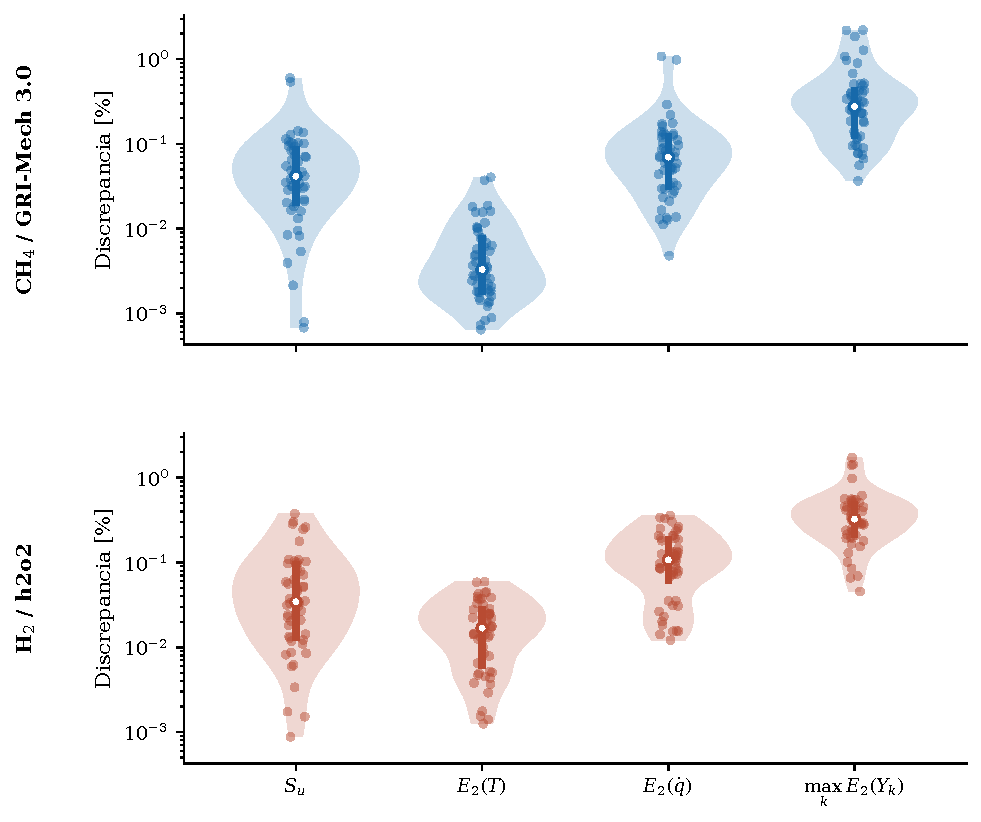
\includegraphics[
    width=\textwidth,
    height=.70\textheight,
    keepaspectratio
]{revision_figures/12_concordancia_global.pdf}
\caption{Concordancia entre \KFLAME{} y \Cantera{} en las 104 condiciones de
la campaña L3. Cada punto representa la mediana de cinco pares de ejecuciones.}
\label{fig:rev-12-concordancia-global}
\end{figure}

\begin{table}[!htbp]
\centering
\footnotesize
\caption{Discrepancias relativas entre \KFLAME{} y \Cantera{} por mecanismo.
Cada celda presenta mediana / percentil 95 / máximo, en \si{\percent}.}
\label{tab:concordance-summary}
\begin{tabular}{@{}lcccc@{}}
\toprule
Mecanismo &
\(\delta_{S_u}\) &
\(E_2(T)\) &
\(E_2(\dot q)\) &
\(\max_k E_2(Y_k)\) \\
\midrule

CH$_4$
& 0.041 / 0.139 / 0.599
& 0.003 / 0.018 / 0.040
& 0.070 / 0.252 / 1.075
& 0.276 / 1.529 / 2.204 \\

H$_2$
& 0.034 / 0.272 / 0.375
& 0.017 / 0.045 / 0.060
& 0.107 / 0.315 / 0.359
& 0.324 / 1.169 / 1.720 \\

\bottomrule
\end{tabular}
\end{table}

La mayor discrepancia de velocidad corresponde al CH$_4$ rico con transporte
multicomponente y Soret, con
\(\delta_{S_u}=\SI{0.599}{\percent}\), mientras que en H$_2$ el máximo alcanza
\SI{0.375}{\percent} a \SI{10}{\atmosphere} con transporte promediado y Soret;
en toda la campaña \(E_2(T)\) permanece por debajo de
\SI{0.060}{\percent}, mientras que las mayores discrepancias relativas se
concentran en los perfiles de especies, con máximos de
\SI{2.204}{\percent} para CH$_4$ y \SI{1.720}{\percent} para H$_2$.

\FloatBarrier

% -----------------------------------------------------------------------------
\subsection{Rendimiento computacional}
\label{sec:L3-performance}
% -----------------------------------------------------------------------------

Una vez extendida la verificación a las 104 condiciones, el análisis se centra
en el rendimiento del proceso completo y en su variación con la composición,
la presión y la temperatura.

\paragraph{Coste del proceso completo}

La razón temporal \(S_t\), definida en la \cref{eq:L3-speedup}, se evalúa en
las 104 condiciones de la campaña, cuyas variables de barrido y condiciones
fijas se recogen en la \cref{tab:campaign-design-L3}; la
\cref{fig:rev-14-speedup-global} proporciona una visión global de la ventaja
temporal relativa entre ambas implementaciones para las variaciones de
composición, presión y temperatura.

\begin{figure}[!htbp]
\centering
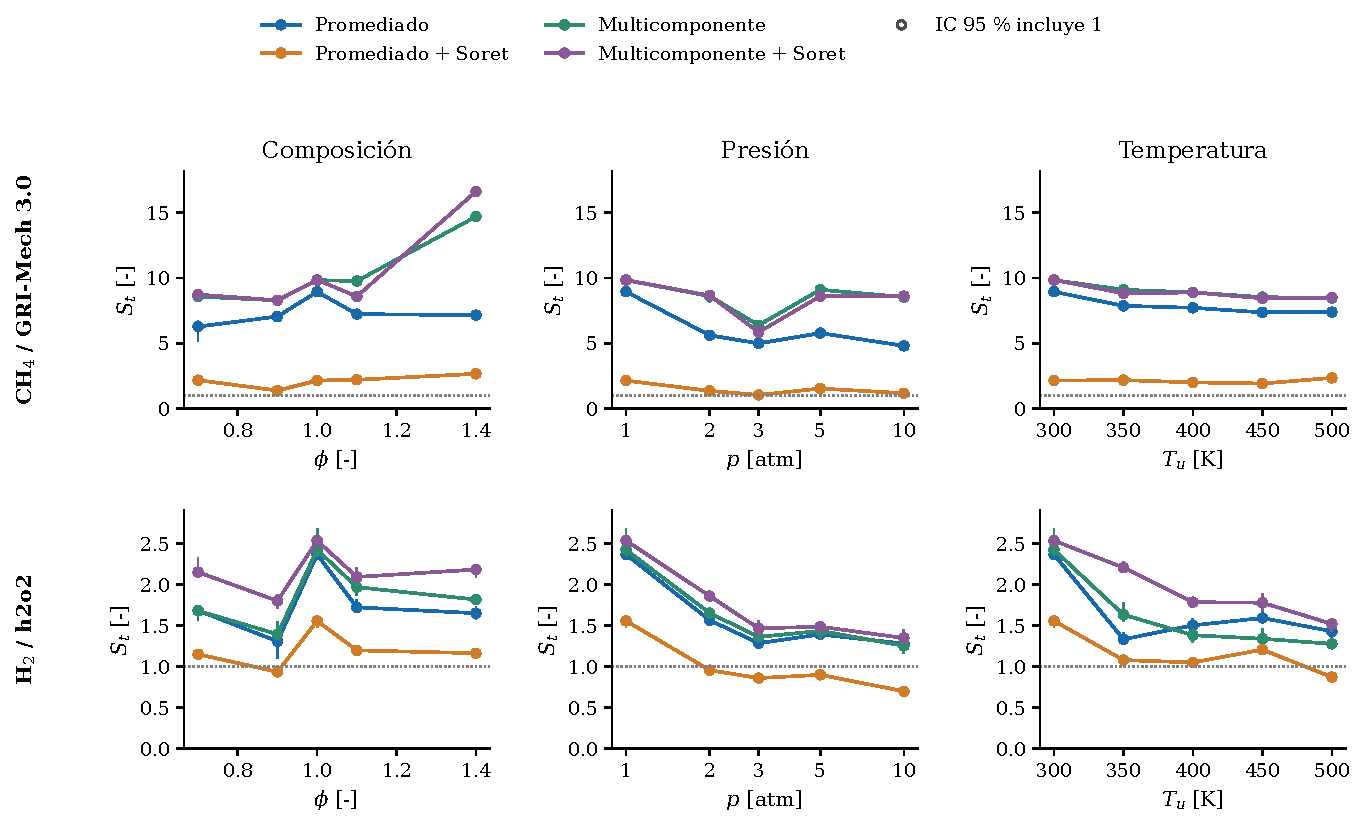
\includegraphics[
    width=\textwidth,
    height=.70\textheight,
    keepaspectratio
]{revision_figures/14_speedup_global.pdf}
\caption{Razón temporal \(S_t\) en las 104 condiciones de la campaña. Las
barras muestran intervalos pareados del 95 por ciento y la línea \(S_t=1\)
representa igualdad de tiempos.}
\label{fig:rev-14-speedup-global}
\end{figure}

En CH$_4$, \(S_t\) varía entre \num{1.04} y \num{16.62}, por lo que las 52
condiciones presentan una mediana temporal menor con \KFLAME{}, mientras que
en H$_2$ el intervalo se reduce a \num{0.70}--\num{2.54} y seis condiciones
presentan una mediana menor con \Cantera{}, todas asociadas al transporte
promediado con Soret. Para observar estas diferencias en términos del tiempo
efectivo de resolución, las
\cref{fig:rev-09-tiempos-composicion,fig:rev-09-tiempos-presion,fig:rev-09-tiempos-temperatura}
desagregan los resultados según cada variable de barrido, manteniendo en cada
caso las condiciones fijas indicadas en la
\cref{tab:campaign-design-L3}.

\begin{figure}[!htbp]
\centering
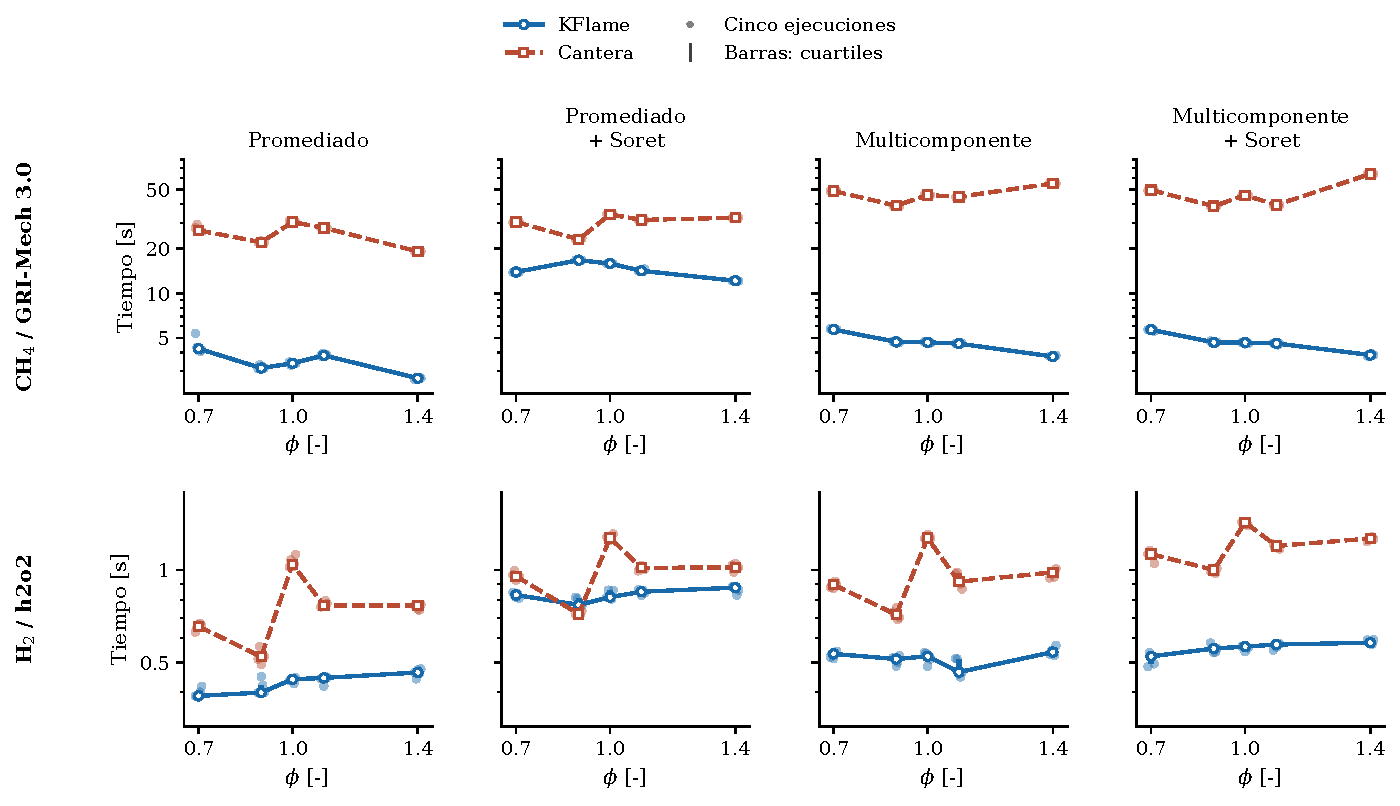
\includegraphics[
    width=\textwidth,
    height=.70\textheight,
    keepaspectratio
]{revision_figures/09_tiempos_transportes.pdf}
\caption{Tiempo de resolución frente a la relación de equivalencia para las
cuatro configuraciones de transporte, con
\(p=\SI{1}{\atmosphere}\) y \(T_{\mathrm{u}}=\SI{300}{\kelvin}\).}
\label{fig:rev-09-tiempos-composicion}
\end{figure}

\begin{figure}[!htbp]
\centering
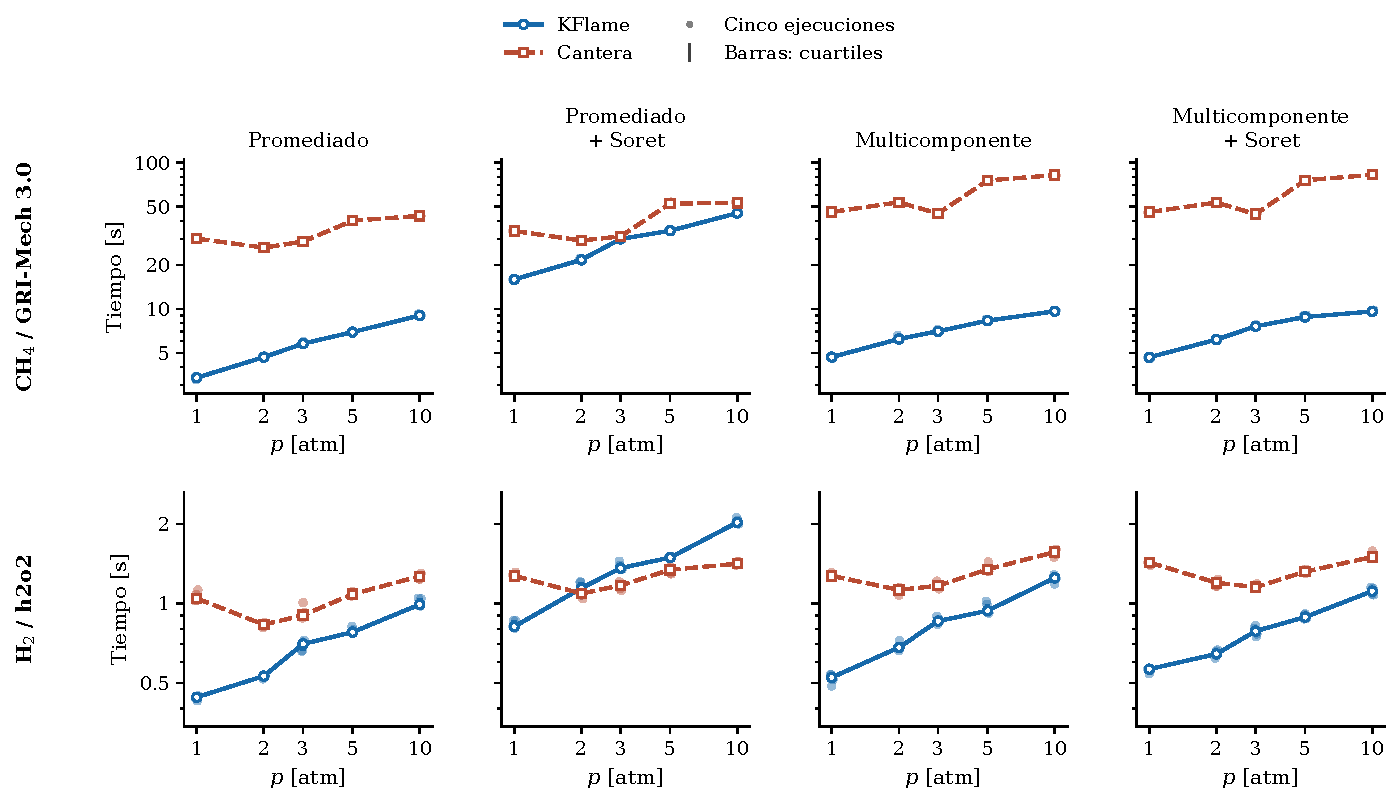
\includegraphics[
    width=\textwidth,
    height=.70\textheight,
    keepaspectratio
]{revision_figures/09_tiempos_presion.pdf}
\caption{Tiempo de resolución frente a la presión para las cuatro
configuraciones de transporte, con
\(\phi=1\) y \(T_{\mathrm{u}}=\SI{300}{\kelvin}\).}
\label{fig:rev-09-tiempos-presion}
\end{figure}

\begin{figure}[!htbp]
\centering
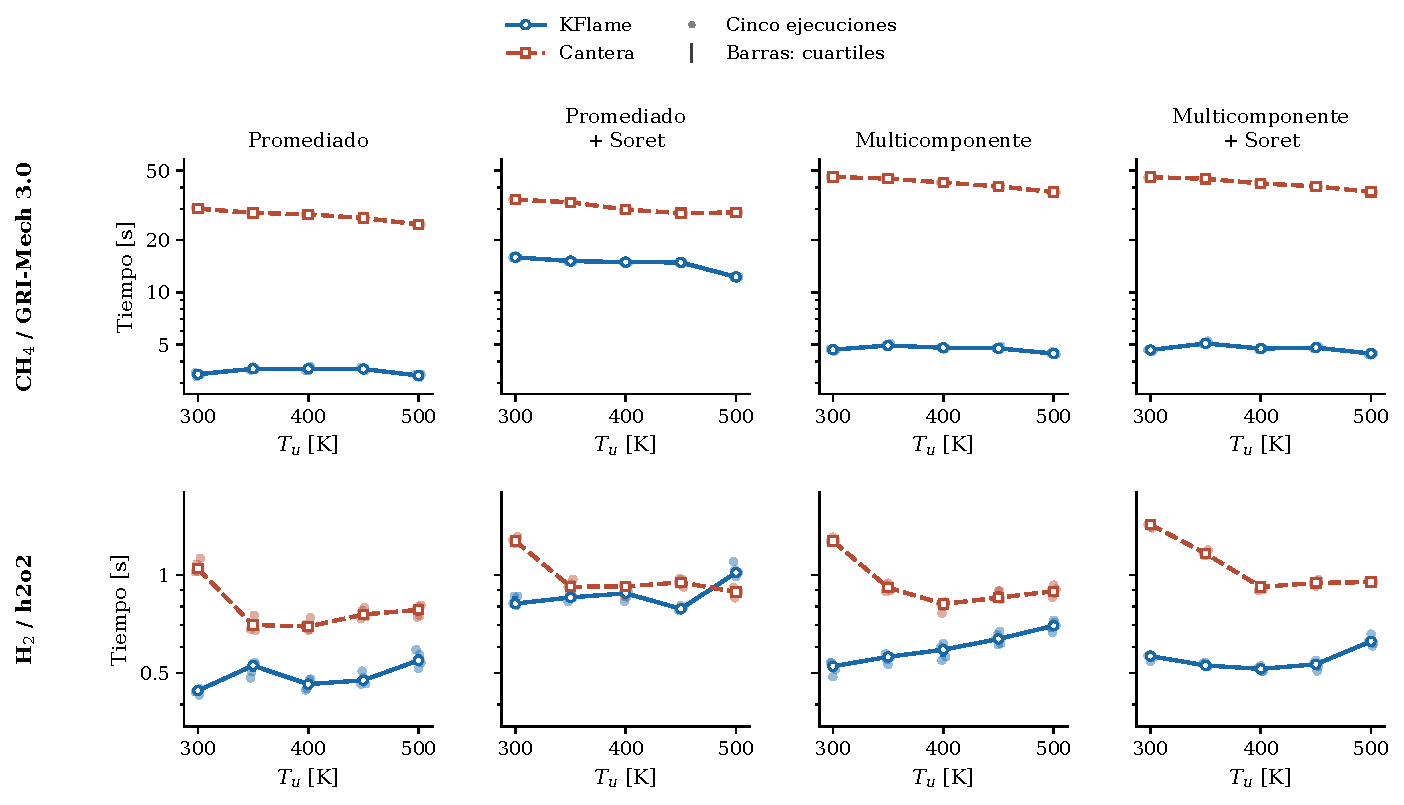
\includegraphics[
    width=\textwidth,
    height=.70\textheight,
    keepaspectratio
]{revision_figures/09_tiempos_temperatura.pdf}
\caption{Tiempo de resolución frente a la temperatura de entrada para las
cuatro configuraciones de transporte, con
\(\phi=1\) y \(p=\SI{1}{\atmosphere}\).}
\label{fig:rev-09-tiempos-temperatura}
\end{figure}

Las tres comparaciones muestran que la diferencia temporal depende tanto del
mecanismo como de la configuración de transporte y de la condición física,
aunque el comportamiento global permanece consistente con la
\cref{fig:rev-14-speedup-global}: la ventaja de \KFLAME{} es más pronunciada
en CH$_4$, mientras que en H$_2$ las diferencias son menores y pueden
invertirse con transporte promediado y Soret; el caso más marcado de esta
inversión aparece a \SI{10}{\atmosphere}, donde la mediana alcanza
\SI{2.03}{\second} en \KFLAME{} y \SI{1.41}{\second} en \Cantera{}.

La comparación temporal se completa con la
\cref{fig:rev-15-precision-speedup}, que relaciona \(S_t\) con la discrepancia
de \(\Su\) definida en la \cref{eq:profile-concordance}, permitiendo comprobar
si las diferencias de coste observadas a lo largo de la campaña se acompañan
de cambios en la concordancia entre ambas implementaciones.

\begin{figure}[!htbp]
\centering
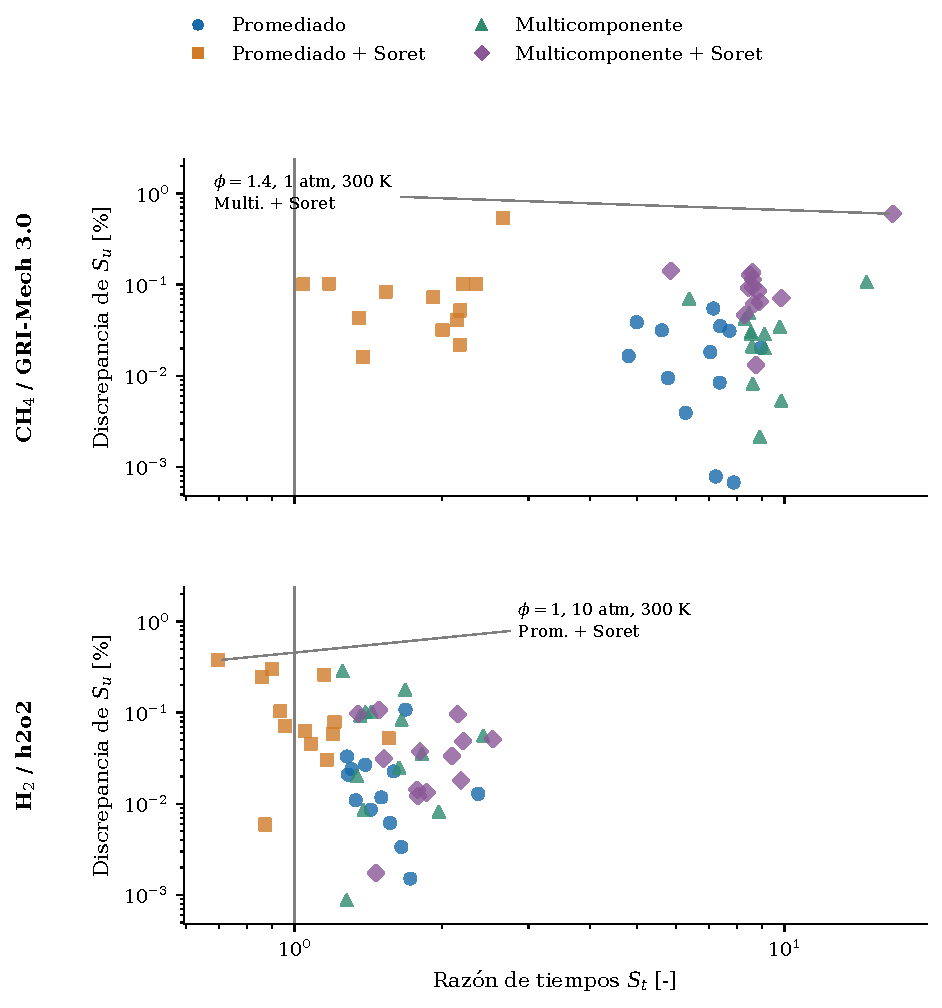
\includegraphics[
    width=\textwidth,
    height=.60\textheight,
    keepaspectratio
]{revision_figures/15_precision_speedup.pdf}
\caption{Discrepancia de \(\Su\) frente a la razón temporal \(S_t\) en las
104 condiciones de la campaña. La línea vertical \(S_t=1\) indica igualdad
de tiempos.}
\label{fig:rev-15-precision-speedup}
\end{figure}

El mayor \(S_t\) corresponde al CH$_4$ rico con transporte multicomponente y
Soret, que presenta también la mayor discrepancia de velocidad; fuera de este
caso no se observa una relación sistemática entre ambas magnitudes, de modo que
las variaciones del coste computacional a lo largo de los tres barridos no
implican por sí mismas una pérdida de concordancia en \(\Su\). En cuanto a la
trayectoria de resolución, ninguna de las 104 condiciones converge mediante
una ruta exclusivamente Newton, ya que las 52 condiciones de CH$_4$ utilizan
PTC y Euler implícito, mientras que las 52 de H$_2$ requieren Euler implícito
sin PTC; el rescate térmico no se activa durante la campaña, la adaptación de
malla interviene en las 104 condiciones y la ampliación del dominio en 101.

\FloatBarrier







\section{FGM}
\label{sec:fgm-results}
% =============================================================================

Una vez verificada la resolución de las llamas individuales, el análisis se
extiende a la construcción completa de tablas FGM para CH$_4$--aire con
GRI-Mech~3.0 y H$_2$--aire con \texttt{h2o2.yaml}. La campaña modifica
únicamente la composición fresca mediante la razón de equivalencia,
\(0.7\leq\phi\leq1.4\), manteniendo aire seco con proporción molar
\(\mathrm{O_2}:\mathrm{N_2}=1:3.76\),
\(T_u=\SI{300}{\kelvin}\),
\(p=\SI{1}{\atmosphere}\) y una anchura inicial del dominio de
\SI{0.03}{\metre}.

Para cada mecanismo se consideran transporte promediado sin Soret, promediado
con Soret, multicomponente sin Soret y multicomponente con Soret, evaluados
tanto con \KFLAME{} como con \Cantera{} de acuerdo con el protocolo de la
\cref{sec:fgm-verification-method}. Se obtienen así ocho construcciones por
mecanismo y dieciséis en total, todas correspondientes a manifolds
bidimensionales \((Z^\star,c)\) a presión y temperatura de entrada fijas.


% =============================================================================
\subsection{Construcción y validación de los manifolds}
\label{sec:fgm-construction-validation}
% =============================================================================

\paragraph{Refinamiento adaptativo}

El criterio de refinamiento de la \cref{eq:fgm-refinement-acceptance} conduce a
una discretización diferente para ambos mecanismos. En CH$_4$ son necesarios
entre 37 y 41 flamelets según el transporte y el solver, mientras que las ocho
construcciones de H$_2$ convergen con 25 dentro del mismo intervalo de
composición. A pesar de esta diferencia, todas las familias finalizan con un
indicador inferior al \SI{1}{\percent} establecido como criterio de aceptación
(\cref{fig:fgm-ch4-refinement,fig:fgm-h2-refinement}), de modo que la mayor
densidad requerida por CH$_4$ responde al refinamiento de su representación y
no a un criterio de convergencia diferente.

\begin{figure}[!htbp]
\centering
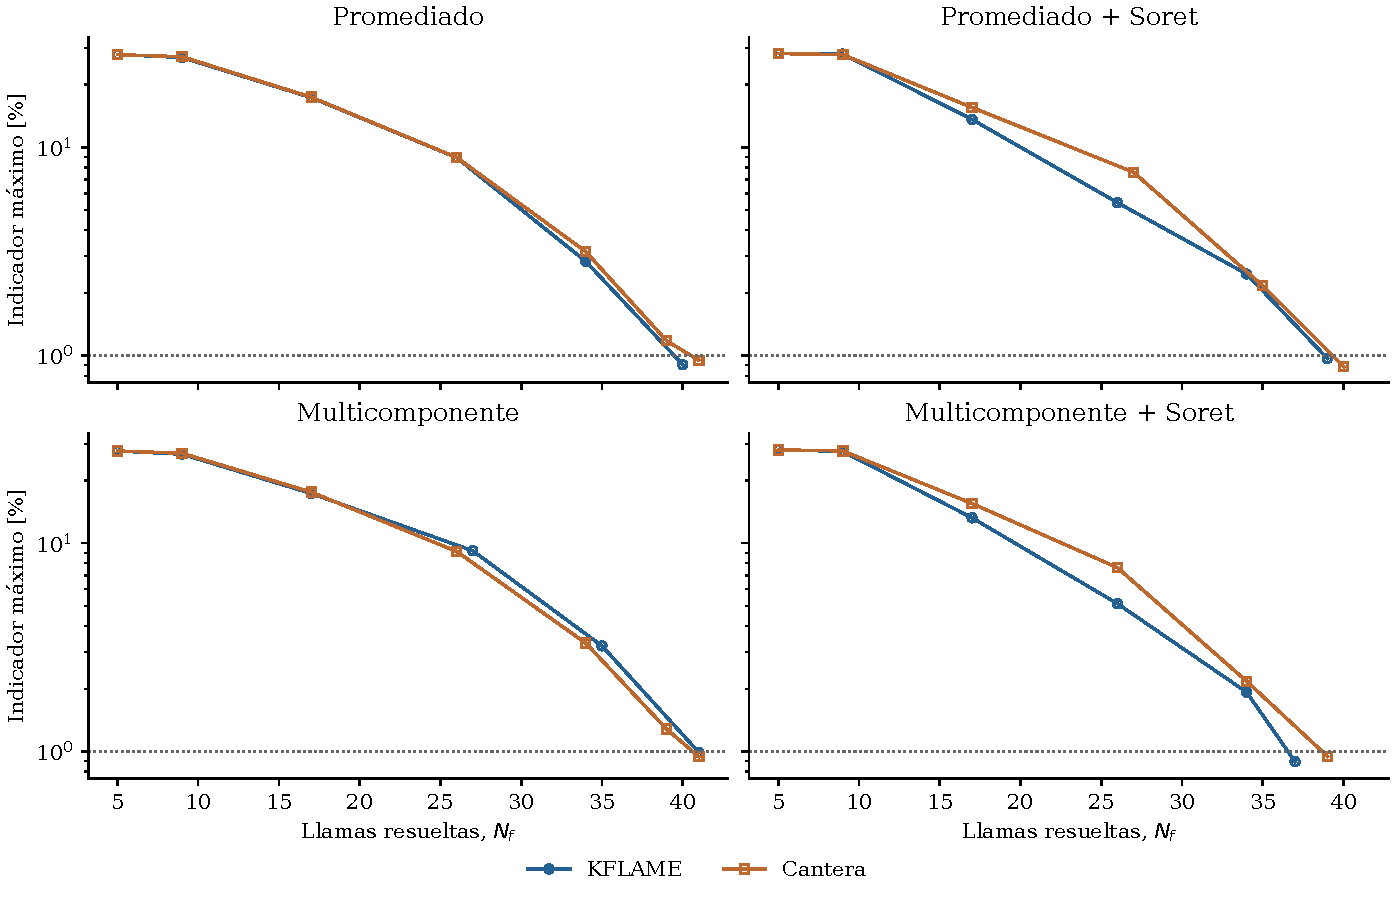
\includegraphics[
    width=\textwidth,
    height=.53\textheight,
    keepaspectratio
]{FGM_FIGURAS/CH4_04_refinamiento.pdf}
\caption{Refinamiento adaptativo de las construcciones FGM de CH$_4$--aire.}
\label{fig:fgm-ch4-refinement}
\end{figure}

\begin{figure}[!htbp]
\centering
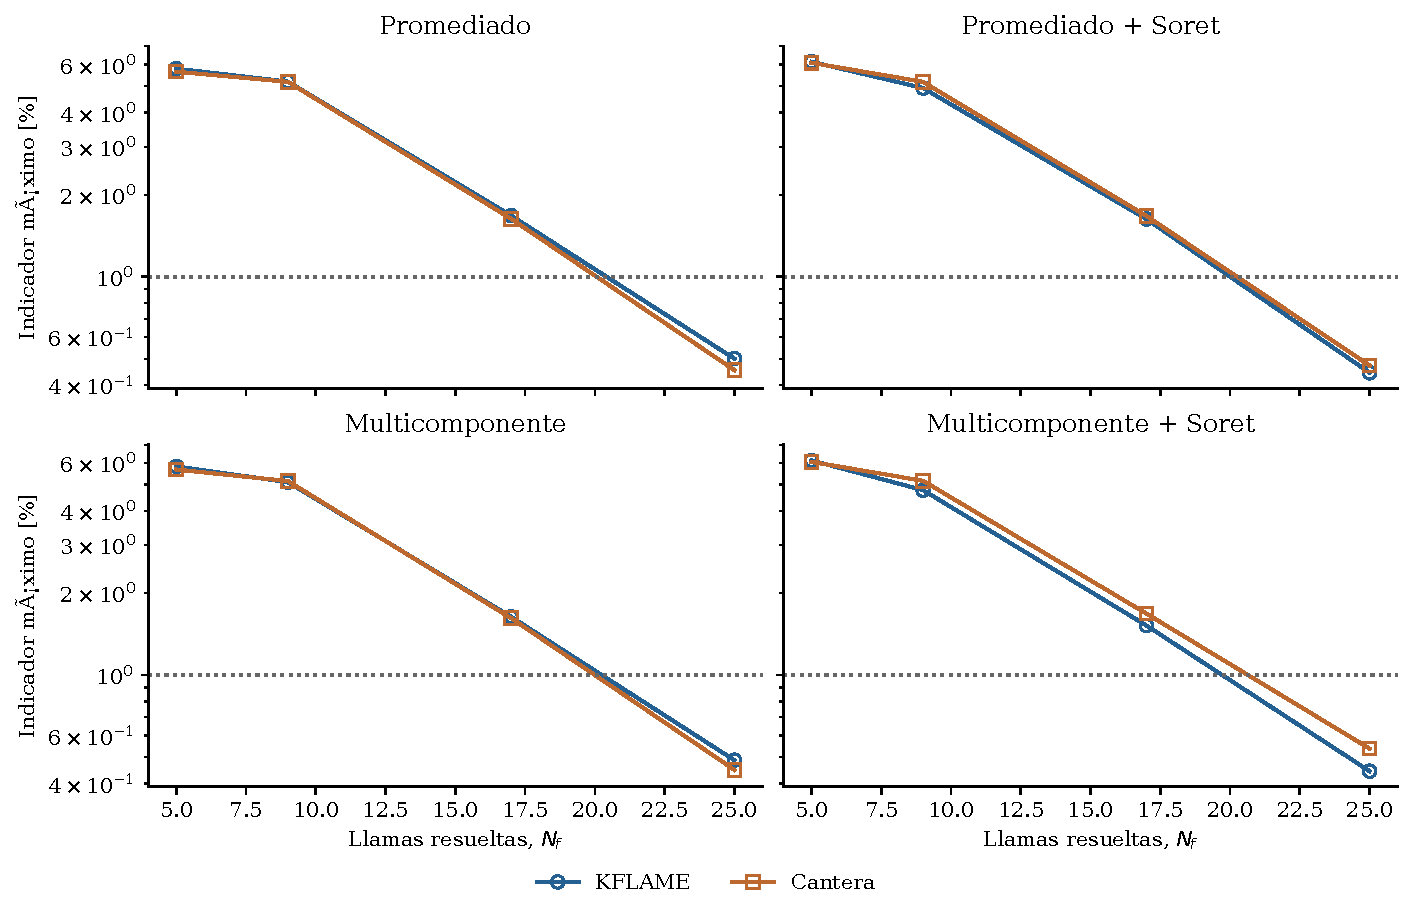
\includegraphics[
    width=\textwidth,
    height=.53\textheight,
    keepaspectratio
]{FGM_FIGURAS/H2_04_refinamiento.pdf}
\caption{Refinamiento adaptativo de las construcciones FGM de H$_2$--aire.}
\label{fig:fgm-h2-refinement}
\end{figure}


\paragraph{Representación del manifold}

La parametrización mediante \(Z^\star\) y la coordenada de progreso definida
en la \cref{eq:progress-c} permite reunir en una superficie bidimensional el
estado termoquímico procedente de la familia de flamelets. Como casos
representativos se emplean las construcciones de \KFLAME{} con transporte
promediado sin Soret; para CH$_4$ se incluyen CO$_2$ y CO, mientras que para
H$_2$ se consideran H$_2$ y O$_2$, junto con la temperatura, velocidad local,
densidad, conductividad térmica, liberación de calor y fuente química de
progreso (\cref{fig:fgm-ch4-map,fig:fgm-h2-map}).

\begin{figure}[p]
\centering
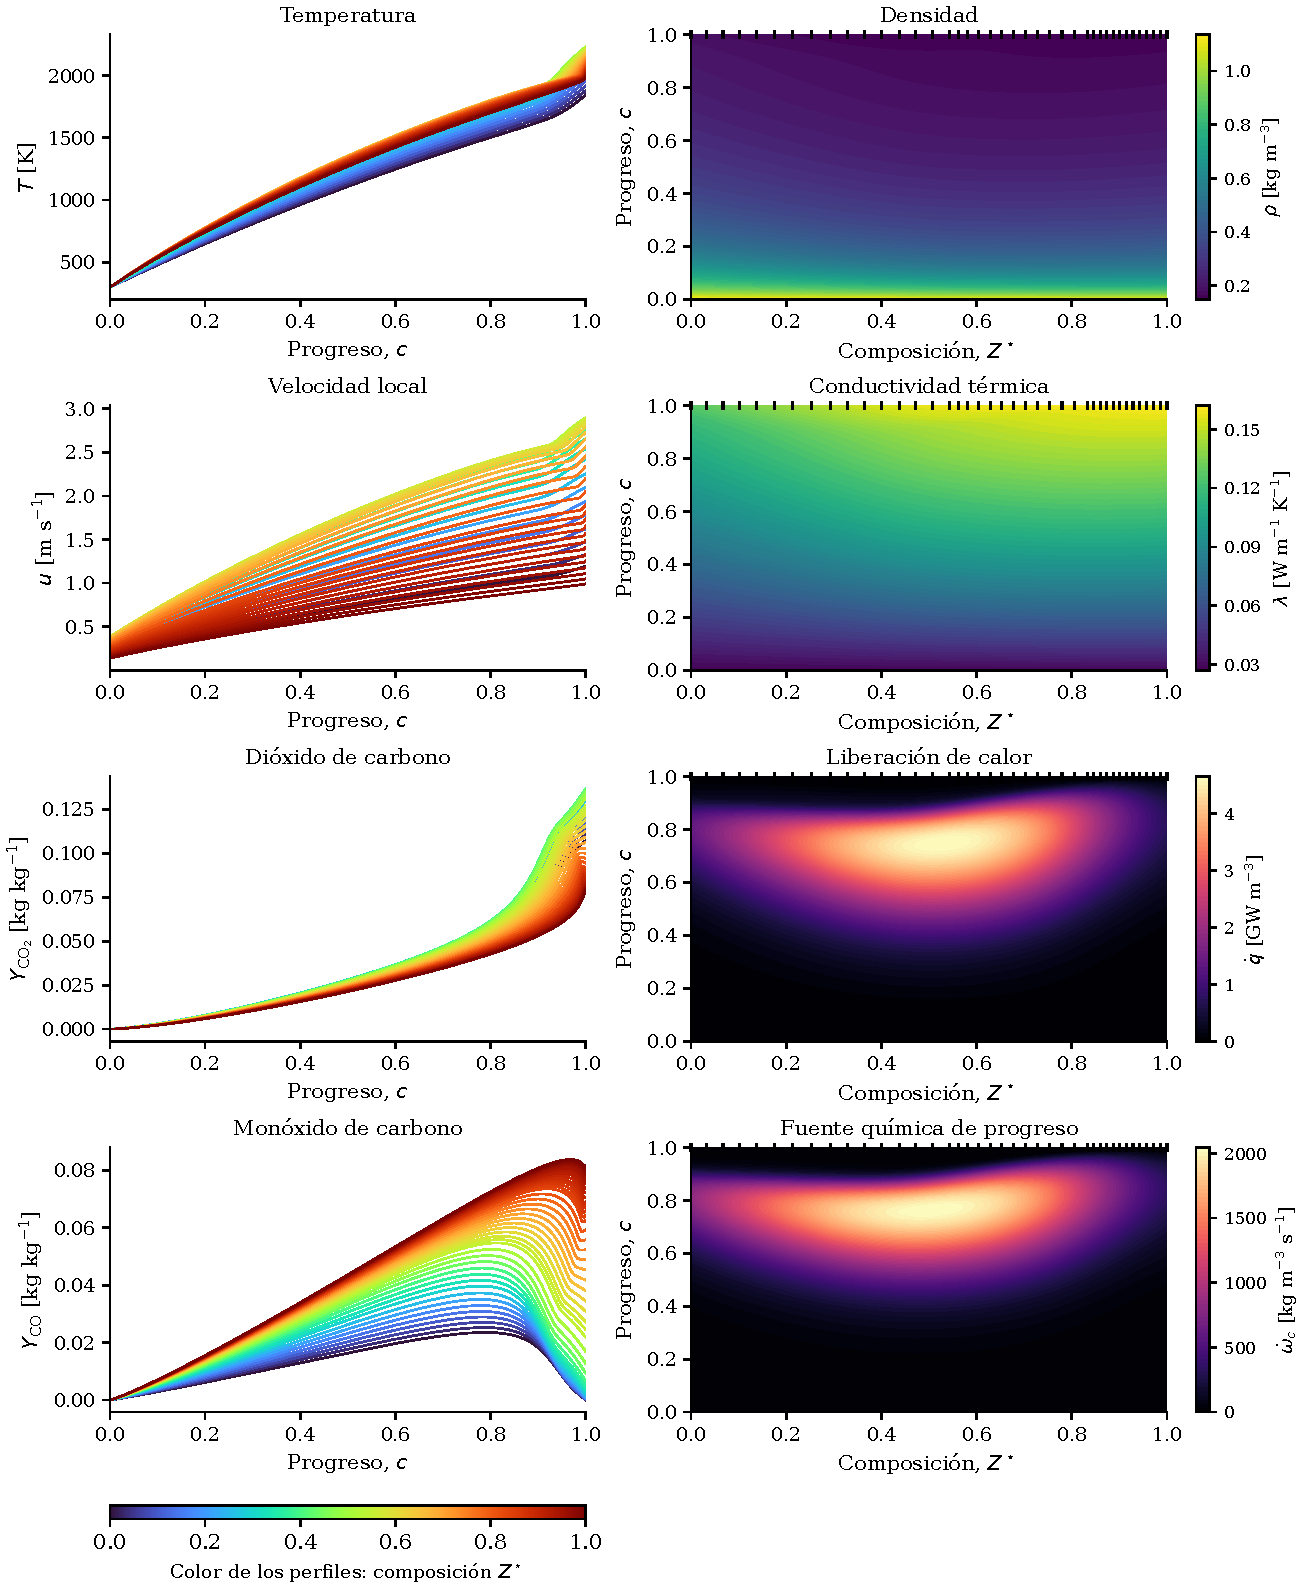
\includegraphics[
    width=\textwidth,
    height=.78\textheight,
    keepaspectratio
]{FGM_FIGURAS/CH4_02_mapa.pdf}
\caption{Manifold FGM representativo de CH$_4$--aire.}
\label{fig:fgm-ch4-map}
\end{figure}

\begin{figure}[p]
\centering
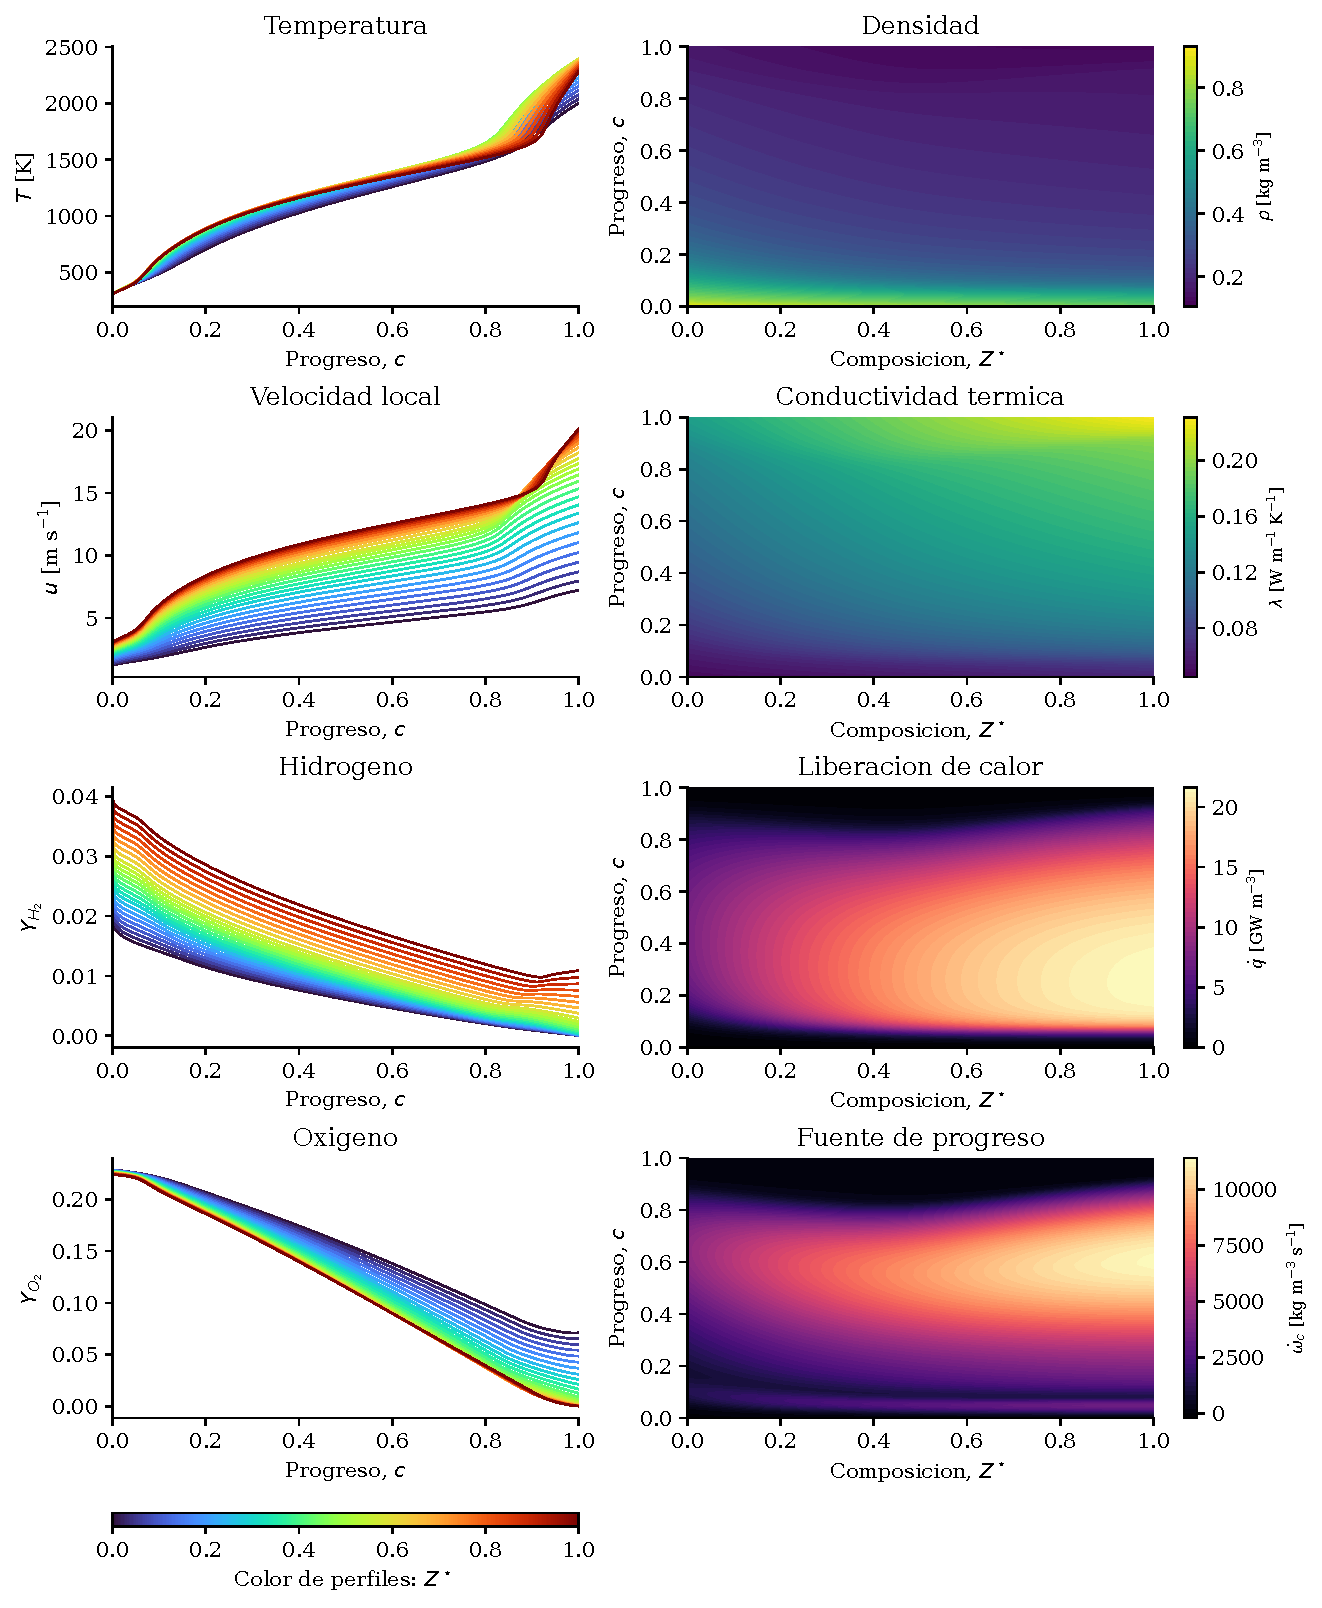
\includegraphics[
    width=\textwidth,
    height=.78\textheight,
    keepaspectratio
]{FGM_FIGURAS/H2_02_mapa.pdf}
\caption{Manifold FGM representativo de H$_2$--aire.}
\label{fig:fgm-h2-map}
\end{figure}


\paragraph{Fidelidad de interpolación}

La capacidad del manifold para reconstruir estados no utilizados durante su
construcción se evalúa con doce llamas retenidas por mecanismo mediante la
\cref{eq:fgm-holdout-error}. En CH$_4$, la temperatura alcanza un P95 de
\SI{0.102}{\percent} y un máximo de \SI{0.423}{\percent}, mientras que la
fuente química de progreso constituye la magnitud más exigente, con
\SI{0.678}{\percent} y \SI{1.22}{\percent}, respectivamente. La medida conjunta
de composición \(e_{Y,2}\) permanece considerablemente por debajo de estos
valores, con un P95 de \SI{0.0599}{\percent} y un máximo de
\SI{0.246}{\percent}, lo que indica que los máximos observados en CO$_2$, CO y
\(\dot{\omega}_c\) corresponden a campos localizados y no a una desviación
simultánea del vector completo de especies
(\cref{fig:fgm-ch4-fidelity,tab:fgm-ch4-errors}).

\begin{figure}[!htbp]
\centering
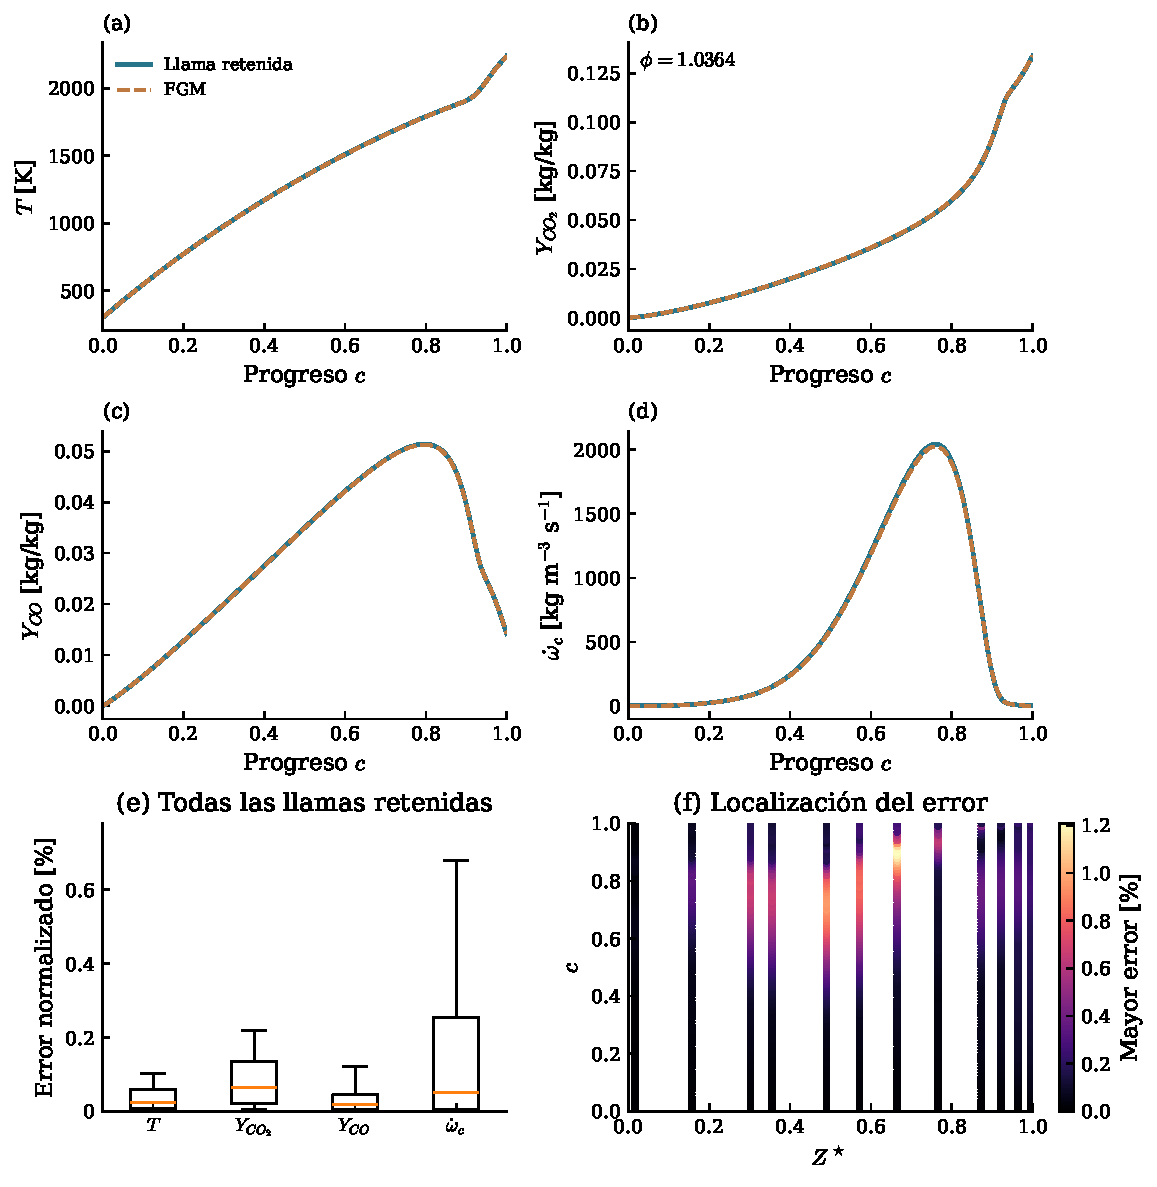
\includegraphics[
    width=\textwidth,
    height=.68\textheight,
    keepaspectratio
]{FGM_FIGURAS/CH4_03_fidelidad.pdf}
\caption{Fidelidad FGM en llamas retenidas de CH$_4$--aire.}
\label{fig:fgm-ch4-fidelity}
\end{figure}

\begin{table}[H]
\centering
\small
\caption{Error de interpolación en llamas retenidas de CH$_4$--aire.}
\label{tab:fgm-ch4-errors}
\begin{tabular}{lrrr}
\toprule
Magnitud & Media [\%] & P95 [\%] & Máximo [\%] \\
\midrule
\(T\)                              & 0.0356 & 0.1020 & 0.423 \\
\(Y_{\mathrm{CO_2}}\)             & 0.0872 & 0.2190 & 1.050 \\
\(Y_{\mathrm{CO}}\)               & 0.0354 & 0.1210 & 0.821 \\
\(e_{Y,2}\) (todas las especies)  & 0.0248 & 0.0599 & 0.246 \\
\(\dot{\omega}_c\)                & 0.1660 & 0.6780 & 1.220 \\
\bottomrule
\end{tabular}

\vspace{0.4em}
\begin{minipage}{0.92\textwidth}
\footnotesize
\textit{Nota:} se emplean doce llamas independientes y 1001 posiciones
uniformes de \(c\) por llama. Los errores se normalizan según la
\cref{eq:fgm-holdout-error}; \(e_{Y,2}\) evalúa conjuntamente el vector completo
de fracciones másicas.
\end{minipage}
\end{table}

Para H$_2$, la reconstrucción mantiene errores del mismo orden y conserva
incluso las estructuras más localizadas. OH presenta el mayor P95 entre las
especies seleccionadas, con \SI{0.225}{\percent}, y un máximo de
\SI{0.803}{\percent}; la fuente química de progreso alcanza
\SI{0.207}{\percent} y \SI{0.779}{\percent}, respectivamente. Sin embargo,
\(e_{Y,2}\) se reduce a \SI{0.0682}{\percent} en el P95 y
\SI{0.132}{\percent} en el máximo, por lo que tampoco se observa una
degradación conjunta de la composición. Los mayores errores permanecen
localizados hacia valores altos de \(c\), particularmente alrededor de
\(Z^\star\simeq0.5\), sin extenderse de forma sistemática al resto del
manifold (\cref{fig:fgm-h2-fidelity,tab:fgm-h2-errors}).

\begin{figure}[!htbp]
\centering
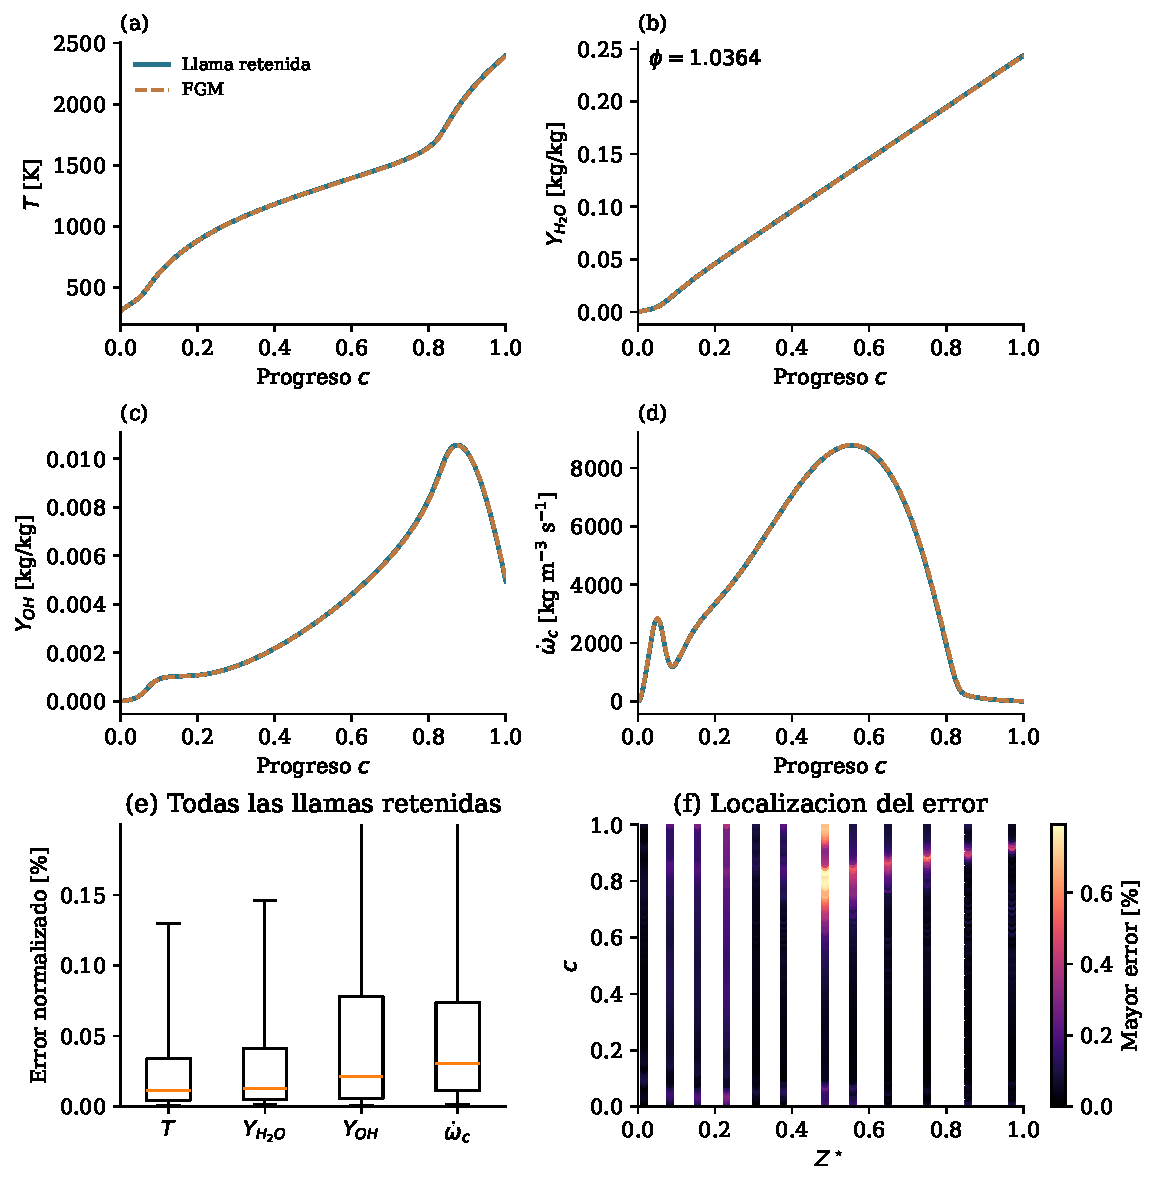
\includegraphics[
    width=\textwidth,
    height=.68\textheight,
    keepaspectratio
]{FGM_FIGURAS/H2_03_fidelidad.pdf}
\caption{Fidelidad FGM en llamas retenidas de H$_2$--aire.}
\label{fig:fgm-h2-fidelity}
\end{figure}

\begin{table}[H]
\centering
\small
\caption{Error de interpolación en llamas retenidas de H$_2$--aire.}
\label{tab:fgm-h2-errors}
\begin{tabular}{lrrr}
\toprule
Magnitud & Media [\%] & P95 [\%] & Máximo [\%] \\
\midrule
\(T\)                              & 0.0302 & 0.1300 & 0.434 \\
\(Y_{\mathrm{H_2O}}\)             & 0.0367 & 0.1460 & 0.283 \\
\(Y_{\mathrm{OH}}\)               & 0.0606 & 0.2250 & 0.803 \\
\(e_{Y,2}\) (todas las especies)  & 0.0179 & 0.0682 & 0.132 \\
\(\dot{\omega}_c\)                & 0.0607 & 0.2070 & 0.779 \\
\bottomrule
\end{tabular}

\vspace{0.4em}
\begin{minipage}{0.92\textwidth}
\footnotesize
\textit{Nota:} se emplean doce llamas independientes y 1001 posiciones
uniformes de \(c\) por llama. Los errores se normalizan según la
\cref{eq:fgm-holdout-error}; \(e_{Y,2}\) evalúa conjuntamente el vector completo
de fracciones másicas.
\end{minipage}
\end{table}


\paragraph{Concordancia entre \KFLAME{} y \Cantera{}}

La validación anterior cuantifica el error introducido por la representación
FGM respecto a flamelets independientes; de forma complementaria, la
\cref{eq:fgm-table-concordance-error} permite determinar cuánto difieren las
tablas obtenidas con ambos solvers bajo una misma configuración de transporte.

En CH$_4$, el P95 de temperatura permanece entre
\SI{0.080}{\percent} y \SI{0.115}{\percent}, mientras que para
\(\dot{\omega}_c\) aumenta hasta \SI{0.916}{\percent} con transporte
multicomponente y Soret. Los máximos puntuales son superiores al P95,
especialmente para la fuente de progreso, donde alcanzan
\SI{2.262}{\percent}; por tanto, las discrepancias mayores se concentran en una
fracción reducida del dominio y no caracterizan el comportamiento global
(\cref{tab:fgm-ch4-concordance}).

\begin{table}[H]
\centering
\small
\caption{Concordancia \KFLAME{}--\Cantera{} para CH$_4$--aire.}
\label{tab:fgm-ch4-concordance}
\begin{tabular}{lrrrr}
\toprule
Transporte &
\(T\) &
\(Y_{\rm CO_2}\) &
\(Y_{\rm CO}\) &
\(\dot{\omega}_c\) \\
\midrule
P
& 0.083 (0.362)
& 0.357 (0.993)
& 0.205 (0.891)
& 0.602 (2.228) \\
P+S
& 0.107 (0.203)
& 0.097 (0.268)
& 0.111 (0.635)
& 0.670 (1.287) \\
M
& 0.080 (0.367)
& 0.382 (1.026)
& 0.252 (0.944)
& 0.610 (2.262) \\
M+S
& 0.115 (0.348)
& 0.248 (0.890)
& 0.146 (0.776)
& 0.916 (2.053) \\
\bottomrule
\end{tabular}

\vspace{0.4em}
\begin{minipage}{0.92\textwidth}
\footnotesize
\textit{Nota:} comparación en \(101\times501\) posiciones comunes de
\((Z_{\rm in},c)\). Cada celda presenta P95 (máximo) del error normalizado,
en porcentaje. Para \(T\) se utiliza como escala el rango térmico de
\Cantera{} y, para las demás magnitudes, el máximo módulo del campo de
referencia. P: promediado; M: multicomponente; S: Soret.
\end{minipage}
\end{table}

En H$_2$, la temperatura mantiene un P95 inferior a
\SI{0.136}{\percent} para las cuatro configuraciones y la fuente de progreso
no supera \SI{0.294}{\percent}. La mayor sensibilidad aparece en OH, cuyo P95
se sitúa entre \SI{0.508}{\percent} y \SI{0.552}{\percent}, con máximos de
hasta \SI{1.723}{\percent}; este comportamiento es consistente con el carácter
más localizado de su distribución frente a especies mayoritarias como
H$_2$O. Aun así, las discrepancias permanecen concentradas y no se trasladan
con la misma magnitud a la temperatura ni a la fuente de progreso
(\cref{tab:fgm-h2-concordance}).

\begin{table}[H]
\centering
\scriptsize
\caption{Concordancia \KFLAME{}--\Cantera{} para H$_2$--aire.}
\label{tab:fgm-h2-concordance}
\begin{tabular}{lrrrrr}
\toprule
Transporte &
\(T\) &
\(Y_{\rm H_2O}\) &
\(Y_{\rm OH}\) &
\(Y_{\rm HO_2}\) &
\(\dot{\omega}_c\) \\
\midrule
P
& 0.095 (0.348)
& 0.202 (0.325)
& 0.552 (1.719)
& 0.062 (0.218)
& 0.247 (0.512) \\
P+S
& 0.119 (0.525)
& 0.249 (0.395)
& 0.508 (1.620)
& 0.091 (0.368)
& 0.250 (0.614) \\
M
& 0.093 (0.317)
& 0.196 (0.305)
& 0.538 (1.723)
& 0.076 (0.244)
& 0.256 (0.484) \\
M+S
& 0.136 (0.407)
& 0.236 (0.377)
& 0.534 (1.677)
& 0.119 (0.512)
& 0.294 (0.505) \\
\bottomrule
\end{tabular}

\vspace{0.4em}
\begin{minipage}{0.96\textwidth}
\footnotesize
\textit{Nota:} cada celda presenta P95 (máximo) del error normalizado, en
porcentaje, sobre una malla común de \((Z_{\rm in},c)\). Para \(T\) se utiliza
el rango térmico de \Cantera{} y, para las demás magnitudes, el máximo módulo
del campo de referencia. P: promediado; M: multicomponente; S: Soret.
\end{minipage}
\end{table}

En conjunto, la prueba de retención y la comparación directa entre solvers
evalúan dos fuentes de error diferentes. La primera confirma que la
interpolación del manifold reproduce estados no utilizados durante la
construcción, mientras que la segunda establece que las diferencias entre
\KFLAME{} y \Cantera{} permanecen pequeñas sobre el dominio tabulado. Los
máximos más elevados se concentran en campos químicos localizados, sin una
degradación equivalente de la temperatura ni del vector global de composición.

\FloatBarrier


% =============================================================================
\subsection{Rendimiento computacional}
\label{sec:fgm-performance}
% =============================================================================

\paragraph{Trayectoria de continuación}

La construcción de una familia FGM no consiste en resolver cada flamelet desde
un estado independiente, sino en aprovechar las soluciones ya convergidas a
medida que se recorre el espacio de composición. En \KFLAME{}, la política de
la \cref{eq:phi-trust-region} utiliza arranques físicos en
\(\phi=0.7\), \(0.9\) y \(1.4\), mientras que las composiciones restantes
reutilizan una solución disponible o emplean el predictor secante. Estos
cambios de inicialización forman parte de la estrategia de continuación y no
representan fallos o recuperaciones del solver.

Para H$_2$, donde las familias finalizan con 25 flamelets, cada construcción de
\KFLAME{} utiliza tres arranques físicos, cuatro reutilizaciones directas y
dieciocho predictores secantes; \Cantera{}, en cambio, emplea un arranque físico
seguido de veinticuatro reutilizaciones del perfil anterior. La diferencia
entre ambas estrategias se refleja en la evolución del coste por flamelet
(\cref{fig:fgm-ch4-family,fig:fgm-h2-family}) y debe considerarse al interpretar
el tiempo acumulado de construcción.

\begin{figure}[p]
\centering
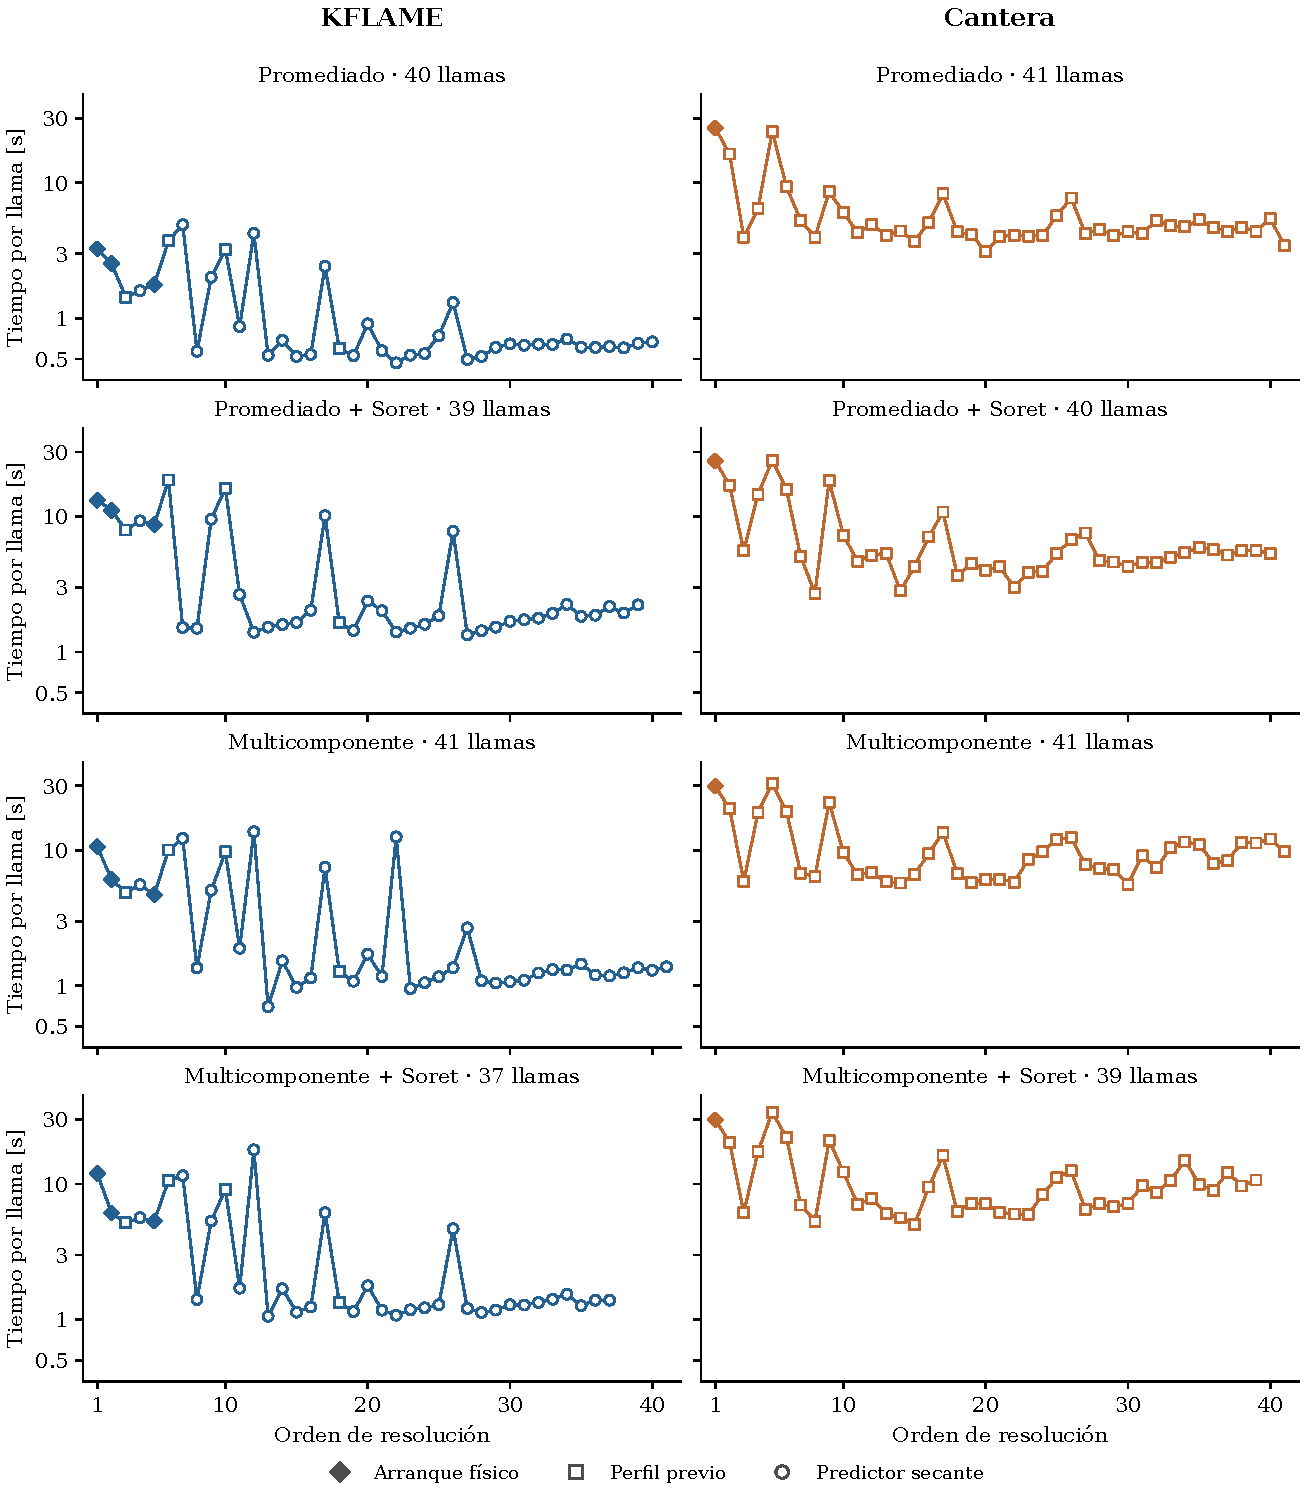
\includegraphics[
    width=\textwidth,
    height=.78\textheight,
    keepaspectratio
]{FGM_FIGURAS/CH4_01_familia.pdf}
\caption{Tiempo por flamelet en las construcciones FGM de CH$_4$--aire.}
\label{fig:fgm-ch4-family}
\end{figure}

\begin{figure}[p]
\centering
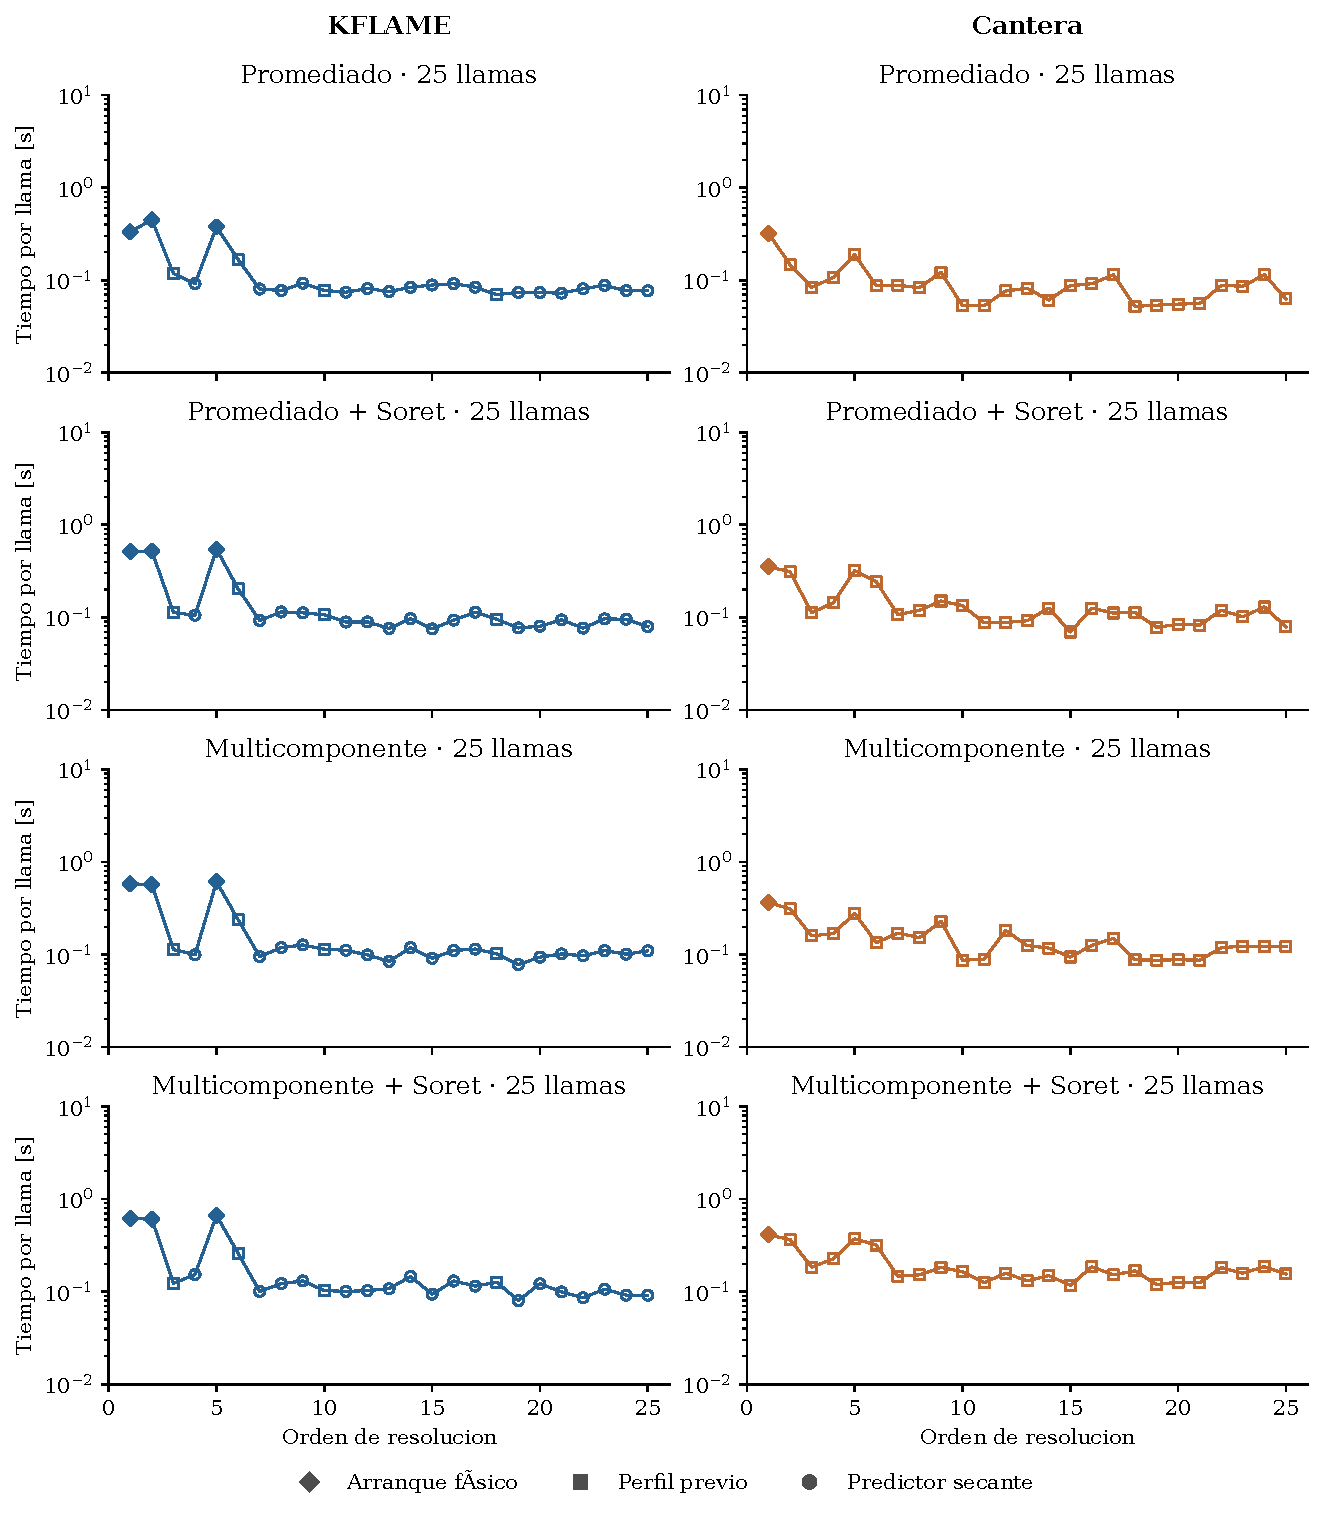
\includegraphics[
    width=\textwidth,
    height=.78\textheight,
    keepaspectratio
]{FGM_FIGURAS/H2_01_familia.pdf}
\caption{Tiempo por flamelet en las construcciones FGM de H$_2$--aire.}
\label{fig:fgm-h2-family}
\end{figure}


\paragraph{Coste total de construcción}

La diferencia de rendimiento depende claramente del tamaño del mecanismo y de
la configuración de transporte. En CH$_4$, \KFLAME{} requiere menos tiempo en
las cuatro configuraciones, con \(S_{\mathrm{FGM}}\) entre \(1.78\) y \(5.07\);
la mayor aceleración corresponde al transporte promediado sin Soret y la menor
al promediado con Soret. En conjunto, las cuatro construcciones requieren
\SI{488.36}{\second} con \KFLAME{} frente a \SI{1412.41}{\second} con
\Cantera{}, lo que corresponde a una razón global de aproximadamente
\(S_{\mathrm{FGM}}=2.89\) y a una reducción acumulada del tiempo del
\SI{65.4}{\percent}.

En H$_2$ la situación se aproxima a la paridad. \KFLAME{} es más lento con
transporte promediado, promediado con Soret y multicomponente, con
\(S_{\mathrm{FGM}}=0.79\), \(0.93\) y \(0.90\), respectivamente, y únicamente
supera a \Cantera{} con transporte multicomponente y Soret, donde alcanza
\(S_{\mathrm{FGM}}=1.06\). El tiempo acumulado de las cuatro configuraciones es
de \SI{15.73}{\second} frente a \SI{14.65}{\second}, por lo que \KFLAME{}
requiere aproximadamente un \SI{7.37}{\percent} más de tiempo y presenta una
razón global \(S_{\mathrm{FGM}}\simeq0.93\). Estas mediciones establecen la
diferencia observada entre ambos solvers, aunque no permiten atribuirla de
forma aislada al mecanismo, al transporte o a la política de continuación.

\begin{figure}[!htbp]
\centering
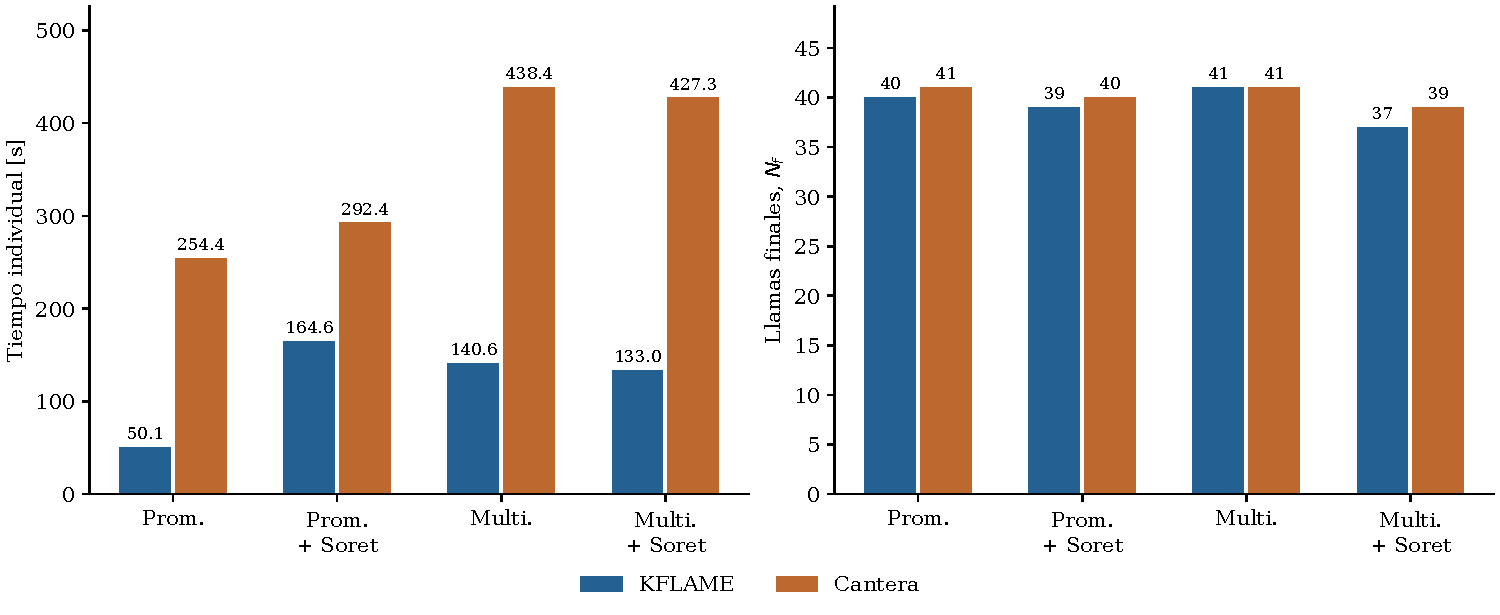
\includegraphics[
    width=\textwidth,
    height=.46\textheight,
    keepaspectratio
]{FGM_FIGURAS/CH4_05_coste_comparado.pdf}
\caption{Coste de construcción de las tablas FGM de CH$_4$--aire.}
\label{fig:fgm-ch4-cost}
\end{figure}

\begin{figure}[!htbp]
\centering
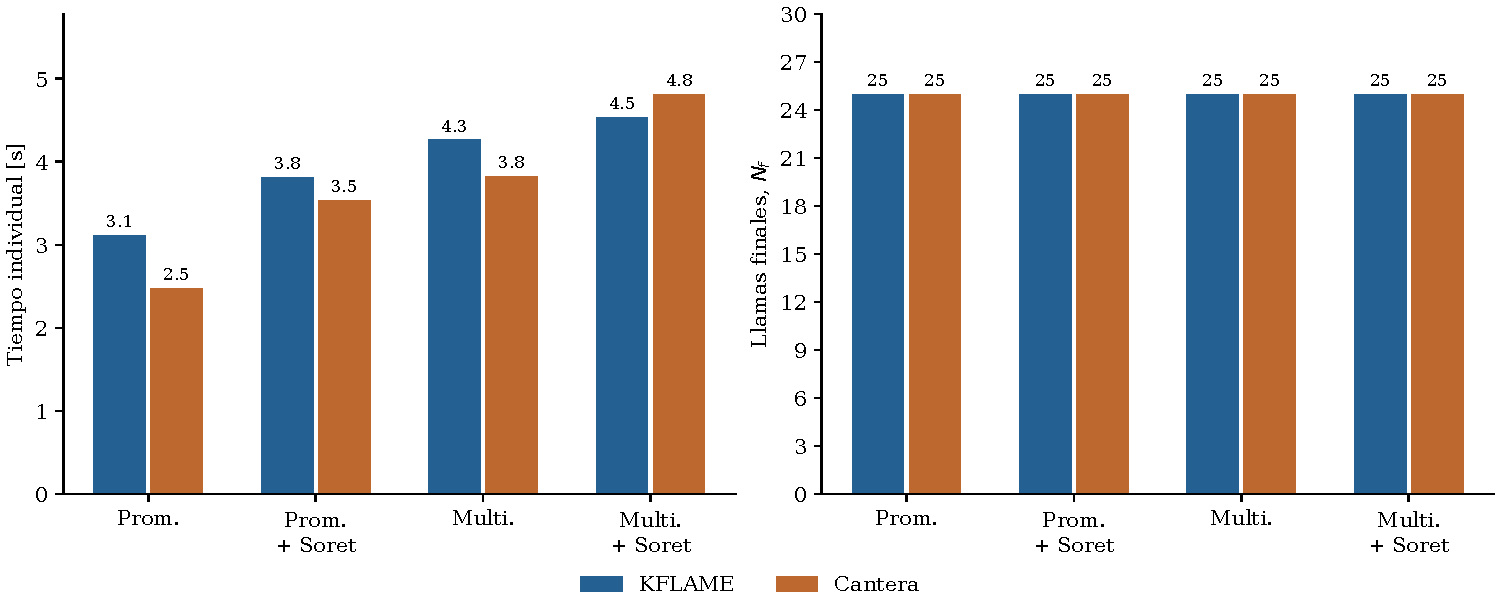
\includegraphics[
    width=\textwidth,
    height=.46\textheight,
    keepaspectratio
]{FGM_FIGURAS/H2_05_coste_comparado.pdf}
\caption{Coste de construcción de las tablas FGM de H$_2$--aire.}
\label{fig:fgm-h2-cost}
\end{figure}

\begin{table}[!htbp]
\centering
\scriptsize
\caption{Coste de construcción de las tablas FGM.}
\label{tab:fgm-construction-cost}
\resizebox{\textwidth}{!}{%
\begin{tabular}{@{}llccccc c@{}}
\toprule
Mecanismo &
Transporte &
\(N_f\) K/C &
\(t_f\) [s] K/C &
\(t_a\) [s] K/C &
\(t_{\mathrm{FGM}}\) [s] K/C &
\(S_{\mathrm{FGM}}\) &
\(d_{\max}\) [\%] K/C \\
\midrule

CH$_4$ & P
& 40 / 41
& 49.64 / 253.81
& 0.48 / 0.48
& 50.13 / 254.37
& 5.07
& 0.903 / 0.948 \\

CH$_4$ & P+S
& 39 / 40
& 164.08 / 291.93
& 0.49 / 0.37
& 164.59 / 292.36
& 1.78
& 0.967 / 0.883 \\

CH$_4$ & M
& 41 / 41
& 140.10 / 437.80
& 0.52 / 0.49
& 140.63 / 438.38
& 3.12
& 0.988 / 0.943 \\

CH$_4$ & M+S
& 37 / 39
& 132.48 / 426.89
& 0.51 / 0.34
& 133.01 / 427.30
& 3.21
& 0.893 / 0.947 \\

\midrule

H$_2$ & P
& 25 / 25
& 3.06 / 2.42
& 0.06 / 0.05
& 3.12 / 2.48
& 0.79
& 0.500 / 0.454 \\

H$_2$ & P+S
& 25 / 25
& 3.76 / 3.48
& 0.05 / 0.05
& 3.81 / 3.54
& 0.93
& 0.444 / 0.472 \\

H$_2$ & M
& 25 / 25
& 4.19 / 3.77
& 0.07 / 0.05
& 4.26 / 3.82
& 0.90
& 0.487 / 0.449 \\

H$_2$ & M+S
& 25 / 25
& 4.47 / 4.76
& 0.06 / 0.05
& 4.54 / 4.81
& 1.06
& 0.444 / 0.537 \\

\bottomrule
\end{tabular}%
}

\vspace{0.4em}
\begin{minipage}{0.96\textwidth}
\footnotesize
\textit{Nota:} K/C corresponde a \KFLAME{}/\Cantera{}; P: transporte
promediado; M: multicomponente; S: Soret. \(N_f\) es el número final de
flamelets, \(t_f\) el tiempo empleado en llamas y propiedades, \(t_a\) el
tiempo de tabulación y selección, y \(t_{\mathrm{FGM}}\) el coste total de
construcción. La razón temporal se define como
\(S_{\mathrm{FGM}}=t_{\mathrm{C}}/t_{\mathrm{K}}\), por lo que valores mayores
que uno favorecen a \KFLAME{}. \(d_{\max}\) corresponde al indicador final de
refinamiento.
\end{minipage}
\end{table}


\paragraph{Consulta de las tablas en memoria}

Una vez construida la tabla, la evaluación termoquímica deja de requerir la
resolución de una nueva llama y se reduce a una interpolación sobre el manifold.
Para la tabla de CH$_4$ generada con \KFLAME{} y transporte promediado, una
consulta aislada requiere una mediana de
\SI{57.605}{\micro\second} por estado, equivalente a
aproximadamente \num{1.74e4} estados por segundo. Al procesar lotes de
\(10\,000\) estados, el coste efectivo disminuye a
\SI{0.203}{\micro\second} por estado y el rendimiento aumenta hasta
aproximadamente \num{4.93e6} estados por segundo.

La consulta por lotes reduce así el coste por estado en un factor cercano a
\(284\) respecto a la evaluación individual. Este factor cuantifica el
beneficio de la ejecución vectorizada del interpolador y no debe interpretarse
como un speed-up de \KFLAME{} frente a \Cantera{} ni como una comparación con
el coste de resolver una llama completa.

\begin{table}[H]
\centering
\small
\caption{Rendimiento de consulta en memoria de la tabla FGM de CH$_4$.}
\label{tab:fgm-query}
\begin{tabular}{rrr}
\toprule
Estados por llamada &
Tiempo por estado [\si{\micro\second}] &
Estados por segundo \\
\midrule
1
& 57.605 [57.039, 59.301]
& \num{1.74e4} \\
10000
& 0.203 [0.203, 0.205]
& \num{4.93e6} \\
\bottomrule
\end{tabular}

\vspace{0.4em}
\begin{minipage}{0.92\textwidth}
\footnotesize
\textit{Nota:} interpolación lineal de \(T\), \(Y_{\rm CO_2}\),
\(Y_{\rm CO}\) y \(\dot{\omega}_c\) sobre la tabla de \KFLAME{} con transporte
promediado. Se muestran mediana \([Q_{25},Q_{75}]\) de cinco mediciones por
tamaño de lote; la preparación del interpolador se excluye del tiempo.
\end{minipage}
\end{table}

\FloatBarrier


\end{document}
